\documentclass[14pt,a4paper,onecolumn]{extarticle}
\usepackage[utf8]{inputenc}
\usepackage{amsmath}
\usepackage{amsfonts}
\usepackage{amssymb}
\usepackage{graphicx}
\usepackage{natbib}
\usepackage{multirow}
\usepackage{pdflscape}

\bibliographystyle{plainnat}
\setlength{\parskip}{1.2em}
\setlength{\parindent}{0pt}
% \graphicspath{{../../images/}}

\author{Ibrahim AbuBakr ElSeddiq}
\title{The predictive value of NT-proBNP on postoperative outcome in patients undergoing offpump CABG}
\begin{document}
\maketitle

\clearpage
\section{Review of Literature}

\subsection{Natriuretic Peptides}

The history of the NP class of biomarkers dates back to 1950s when early electron microscopy studies reported dense granules in the atrial myocardium similar to glandular tissue from endocrine organs. Soon, the close interplay between atria and intravascular volume was revealed; stretching of canine left atrium increased urine output and injection of atrial tissue into rats caused diuresis and natriuresis. Atrial natriuretic peptide (ANP) was subsequently purified, sequenced, and reproduced. \citep{Gaggin2014} %PHYSIOLOGY%


B-Type natriuretic peptide was discovered in 1988. Proof of the existence of amino-terminal pro–B-type natriuretic peptide (NT-proBNP) in the human circulation and its relationship to cardiac function were first reported by Hunt and colleagues in 1995. \citep{Richards2018} %PHYSIOLOGY

The biological actions of the cardiac natriuretic peptides (NP) indicate they constitute an endogenous compensatory system that acts to counter excess cardiac load and volume expansion. Actions include natriuresis, diuresis, vasodilation, and lusitropism, plus direct suppression of volume-retaining, vaso-constricting systems including the renin–angiotensin–aldosterone and sympathetic nervous systems. NP also have trophic actions opposing cardiac hypertrophy and fibrosis. \citep{Richards2018} %PHYSIOLOGY

Cardiac chamber wall stress, the prime driver of NP synthesis and release, in accord with the law of Laplace, is directly related to intrachamber pressure and chamber radius and inversely related to wall thickness. In concentrically hypertrophied hearts, as commonly observed in patients with HF with preserved ejection fraction (HFpEF), unit wall stress is less than in those patients with HF with reduced ejection fraction (HFrEF) and dilated left ventricles. Accordingly, plasma NP in acute decompensated HF (ADHF) are lower in HFpEF compared with HFrEF. NT-proBNP is correlated with several echocardiographic indicators of cardiac structure and function including: \begin{itemize}   \item Left ventricular (LV) end-diastolic wall stress   \item LV ejection fraction (LVEF)   \item E/e’   \item LV longitudinal strain   \item LV circumferential strain   \item Left atrial dimensions   \item Right ventricular ejection fraction   \item Right ventricular pressures \end{itemize} \citep{Richards2018} %DIAGNOSIS

Iwanaga and colleagues measured systolic and diastolic wall stress by echocardiography and cardiac catheterization, and related this key measurement to plasma concentrations of NP in patients with HF. A striking correlation between plasma BNP with end-diastolic wall stress (r 2 5 0.887; P<0.001) seemed to be far stronger than the correlation with LV end-diastolic pressure (r 2 5 0.296; P<.001). NP levels seem to reflect LV wall stress more closely than other ventricular parameters in HF, and this relationship may better account for interindividual differences in plasma NP values than other measures. \citep{Iwanaga2006} %DIAGNOSIS

Plasma NP concentrations reflect aspects of diastolic dysfunction independent of age, sex, renal function, body mass index, and LVEF. Plasma NT-proBNP (>600 pg/mL) and BNP (>100 pg/mL) are strong, albeit relatively nonspecific, independent predictors of restrictive filling the most severe grade diastolic dysfunction. In HF, plasma NT-proBNP correlates with E/e’, a well-validated index of LV filling pressures, in addition to measures of LV compliance, myocardial relaxation, and left atrial dimensions. With respect to right heart function, plasma concentrations of B-type NPs are inversely related to right ventricular ejection fraction and directly related to right ventricular dimensions and estimated intraventricular pressures. \citep{Troughton2009} %DIAGNOSIS

An echocardiographic substudy of the phase II PARAMOUNT trial (LCZ696 Compared to Valsartan in Patients With Chronic Heart Failure and Preserved Left-ventricular Ejection Fraction) of valsartan-sacubitril therapy in HFpEF, demonstrated decreases in LV systolic longitudinal and circumferential strain that were significantly related to plasma NT-proBNP independent of age, sex, systolic and diastolic blood pressures, body mass index, LVEF, left atrial volume index, E/E’, atrial fibrillation (AF), or renal function. \citep{Kraigher-Krainer2014} %DIAGNOSIS %PHYSIOLOGY

The relationship between cardiac structure and function and associated cardiac transmural distending pressures and myocyte stretch on the one hand with cardiac release and plasma concentrations of NT-proBNP on the other underpins the strength of NT-proBNP as a biomarker in HF. NT-proBNP has good diagnostic performance for discrimination of acute heart failure among patients presenting with new-onset dyspnea. \citep{Richards2018} %DIAGNOSIS

In this setting the relationship of NT-proBNP to intracardiac pressures and HF status, plasma is undistorted, whereas BNP is no longer a reliable marker. NT-proBNP but not BNP remains a valid marker during ARNI therapy. Where ARNI therapy is contemplated or already in place, NT-proBNP is the marker of choice in assessment of possible incident ADHF and for serial monitoring. \citep{Richards2018} %LIMITATIONS

However, elevation of plasma NT-proBNP is not specific for ADHF. AF, renal failure, pulmonary embolism, and a number of other causes increase NT-proBNP (Box 1). NT-proBNP level should be considered in concert with the clinical history, examination findings, and data from other tests, including a standard laboratory workup and cardiac imaging. Age, obesity, preserved ejection fraction, renal dysfunction, and AF may affect the diagnostic performance of NT-proBNP. \citep{Richards2018} %LIMITATIONS

Consideration of confounding influences on NP plasma concentrations is necessary for interpretation ofplasma NT-proBNP results in those with mild or early decompensated HF, or in epidemiologic settings where elevation of median plasma concentrations is not profound and background confounders become more intrusive. \citep{Richards2018} %LIMITATIONS

Age is a strong determinant of NT-proBNP. This relationship is independent of kidney and cardiac function, and the exact underlying mechanisms remain unclear.  \citep{Richards2018} %LIMITATIONS

Age-adjusted values enhance the specificity and accuracy of NT-proBNP in diagnosis of ADHF at the cost of some loss of sensitivity. An NT-proBNP level of 450 pg/mL or more in the presence of new onset dyspnea is highly discriminating for ADHF (AUC, 0.99) in those less than 50 years of age. Most HF patients are older and the AUC falls progressively to 0.93 and then 0.86 in patients aged 50 to 75 years (optimal threshold of 900 pg/mL) and those older than 75 years (1800 pg/mL), respectively. Age-adjusted values have been calculated for NT-proBNP but not BNP. \citep{Januzzi2006a} %LIMITATIONS

The typical elevation of plasma NT-proBNP in the setting of severe symptomatic ADHF is so pronounced (median values are >5000 pg/mL and are typically >40-fold greater than the levels observed in controls without HF) that this marker achieves an excellent “signal-to-noise ratio” for ADHF. LV structure and function influence plasma NT-proBNP. Specifically, plasma NT-proBNP plasma concentrations in HFpEF are approximately half those observed in HFrEF in both acute and chronic HF. This reflects the integrated influence of ventricular internal dimensions, wall thickness, and intraventricular pressures (embodied in the law of Laplace) on unit wall stress and cardiomyocyte stretch, the primary driver of NP synthesis and release. In the setting of incipient or treated HF, NP values often fall into the subdiagnostic range and this is particularly so in HFpEF. This emphasizes the need to apply the recommended cutpoint values for acute HF in the appropriate setting; that is, with new onset of distressing breathlessness where acute HF is likely. When NPs fall into the “gray zone” between rule out and rule in values for acute HF echocardiography is an invaluable diagnostic adjunct with elevated E/e’ and/or the presence of a restrictive filling pattern helping securing the diagnosis of HF. \citep{Richards2018} %DIAGNOSIS

The ICON study (International Collaboration on NT-proBNP) included data on 1256 patients presenting with new-onset shortness of breath. ICON data defined the sensitivity, specificity, negative predictive value, positive predictive value, and overall accuracy of NT-proBNP for the diagnosis of acute HF in acutely symptomatic patients.  Plasma NT-proBNP of 300 pg/mL acts as an excellent rule-out threshold with a sensitivity for ADHF consistently greater than 90\%. A plasma NT-proBNP of less than this threshold indicates symptoms are highly unlikely to be due to acute heart failure. Acutely symptomatic patients with a NT-proBNP of less than 300 pg/mL are very unlikely to have acute heart failure. Specificity is improved by using age-specific cutpoints with 450, 900, and 1800 pg/mL performing well for age groups less than 50, 50 to 75, and greater than 75 years, respectively. \citep{Januzzi2006a} %DIAGNOSIS

\begin{figure}   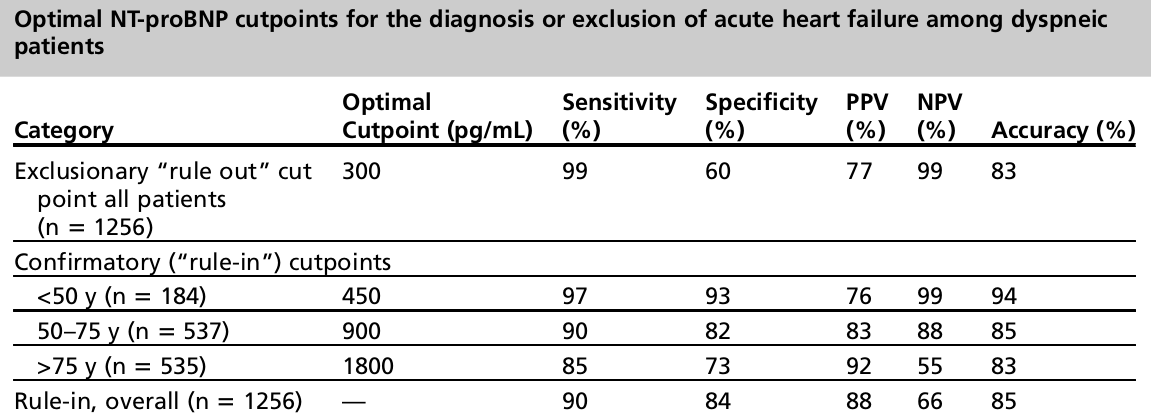
\includegraphics{../../images/NTBNP_cutpoints.png}   \caption{Abbreviations: NT-proBNP, amino-terminal pro–B-type natriuretic peptide; NPV, negative predictive value; PPV, positive predictive value.\citep{Januzzi2006a}}   \label{NTBNP_cutpoints} \end{figure} %DIAGNOSIS

\begin{figure}   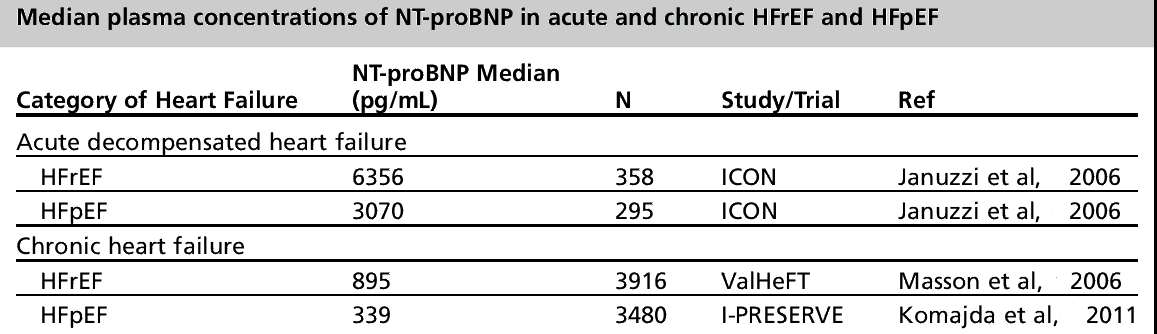
\includegraphics{../../images/NTBNP_HF.png}   \caption{Abbreviations: HFpEF, heart failure with preserved left ventricular ejection fraction; HFrEF, heart failure with reduced left ventricular ejection fraction; NT-proBNP, amino-terminal pro–B-type natriuretic peptide. \citep{Richards2018}}   \label{NTBNP_HF} \end{figure} %DIAGNOSIS

The 2016 European Society of Cardiology guidelines for the diagnosis and management of heart failure strongly mandate measurement of NT-proBNP in the diagnostic workup for suspected acute heart failure emphasizing a rule out threshold of 300 pg/mL. \citep{Ponikowski2016} %DIAGNOSIS

Therapy with combined angiotensin 2 type1 receptor blockade and neprilysin inhibition (ARNI) has recently been shown to be superior to treatment with angiotensin-converting enzyme inhibition in chronic heart failure, offering an approximate 20\% improvement in all key important clinical endpoints. \citep{McMurray2014} %TREATMENT

Neprilysin mediates cleavage of the biologically active carboxy terminals of ANP, BNP, and C-type NP, and prolongation of the circulating and tissue half-lives of these powerful effectors is presumed to underlie a significant proportion of the benefit offered by ARNI. \citep{Bayes-Genis2016} %TREATMENT

Prescription of ARNI in chronic HF resulted in sustained elevations in plasma BNP, whereas NT-proBNP (which is not cleaved by neprilysin) decreased, reflecting impaired metabolism of carboxy terminal BNP and decreased cardiac release of NP, respectively. \citep{Packer2015} %TREATMENT

In a study of 305 patients assessed by 92 family doctors for suspected incipient heart failure (on the basis of exertional dyspnea and/or peripheral edema), the addition of plasma NT-proBNP measurements to clinical history and examination, significantly improved diagnostic accuracy by 10 patients per 100 assessed. \citep{bib3133} %DIAGNOSIS

AF increases plasma NT-proBNP whether HF is present or not. AF is a common complication of HF, and occurs in approximately 30\% of populations with ADHF. AF reduces the discriminative performance NT-proBNP for newly symptomatic ADHF, reducing the AUC on receiver operator analysis to approximately 0.7, which is well below the approximately 0.9 observed in HF cases with preserved sinus rhythm.  The sensitivity of the standard thresholds of NT-proBNP are preserved in the face of overall increases in plasma peptide concentrations, but specificity and accuracy are clearly reduced and cannot be improved solely by selection of an alternative cut point. Empirical observation indicates that between 65\% and 85\% of acutely breathless patients with AF and NT-proBNP levels of greater than 300 pg/mL will receive a final diagnosis of acute HF and they should be managed as such until an alternative diagnosis is proven.  \citep{Richards2013} %LIMITATIONS

Obesity lowers plasma NP concentrations through poorly understood mechanisms. Body mass index is actually inversely related to plasma NT-proBNP concentrations in both health and HF. Unlike renal impairment or AF, which irretrievably impair the specificity and accuracy of plasma NT-proBNP, obesity shifts the optimal threshold but preserves discriminatory performance. The effect on the diagnostic performance of BNP at 100 pg/mL is pronounced, with a clear loss of sensitivity that has led to the recommendation to reduce the cutpoint to 50 pg/mL for those with a BMI greater than of 30 kg/m 2. \citep{Daniels2006} %LIMITATIONS

\begin{figure}   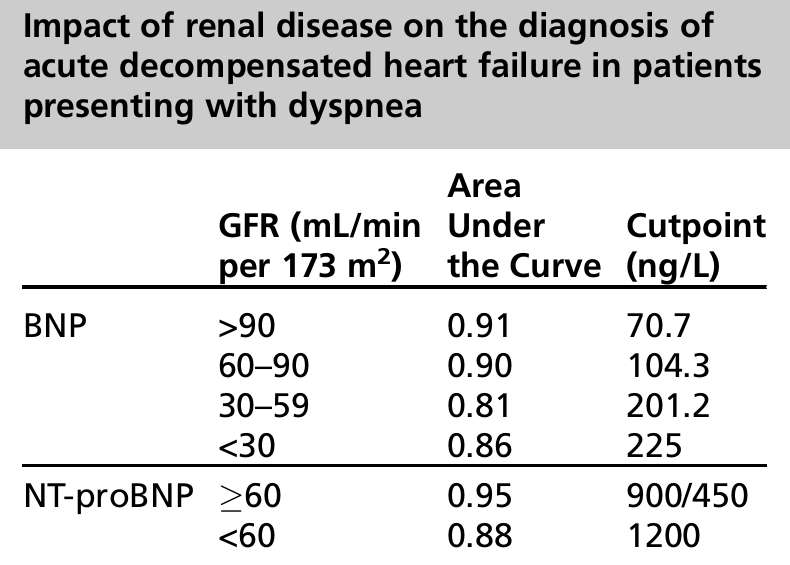
\includegraphics{../../images/NP_obesity.png}   \caption{Abbreviations: BNP, B-type natriuretic peptide; GFR, glomerular filtration rate; NT-proBNP, amino-terminal pro–B-type natriuretic peptide. \citep{DeFilippi2008}}   \label{NP_obesity} \end{figure} %LIMITATIONS %DIAGNOSIS


Estimated glomerular filtration fraction rate are inversely related to plasma concentrations of BNP and NTproBNP. For BNP, this has led to the recommendation that the BNP threshold be increased to 200 pg/mL for an estimated glomerular filtration rate of less than 60 mL/min/1.73 m. No specific corresponding change in cut-point is generally applied to NT-proBNP values and the performance of age-specific NT-proBNP diagnostic thresholds seem to be less affected. \citep{DeFilippi2008} %LIMITATIONS %DIAGNOSIS

The ValHeFT therapeutic trial (Valsartan Heart Failure Trial) in chronic HFrEF generated a large neurohormonal substudy providing excellent data on the prognostic performance of both NT-proBNP and BNP in chronic heart failure with reduced LVEF.  After comprehensive adjustment for demographic, biochemical, clinical, and imaging predictors, NT-proBNP remained an independent predictor of all-cause death and of readmission for HF. NT-proBNP performed more strongly than endothelin, aldosterone, or norepinephrine. Median plasma NT-proBNP concentrations of 895 pg/mL corresponded with an unadjusted crude annual mortality of approximately 10.1\%. Increments of 500 pg/mL in NT-proBNP conferred a 3.0\% to 3.8\% increment in risk of all-cause death or HF readmission. From first to tenth deciles of NT-proBNP, the ValHeFT population exhibited a 10-fold range in risk of all-cause death, HF readmission and the composite endpoint. \citep{bib3204} %PROGNOSIS

A large number of HF patients (n=4128) participated in the marker substudy from the I-PRESERVE therapeutic trial (Irbesartan in Heart Failure With Preserved Systolic Function) of irbesartan in HFpEF. Plasma NT-proBNP concentrations were related to outcomes, including 1515 episodes of all-cause death cardiovascular admission, 881 deaths, and 716 HF deaths/HF admissions. A median NT-proBNP of 339 pg/mL conferred a crude unadjusted annual mortality of 5.1\%. In comprehensive multivariate modeling, NT-proBNP was the strongest independent predictor of outcomes at 3 years of follow-up. Across septiles of NT-proBNP, risk extended over 7- to 20-fold ranges from 8.1\% to 59.9\% for the primary endpoint, 2.7\% to 36.5\% for death and 2.1\% to 38.9\% for HF death/HF admission. NT-proBNP, independent of multiple other accepted predictors, provided fine-grained prediction of clinical outcomes from low to very high risk. \citep{Komajda2011} %PROGNOSIS

In the landmark PARADIGM trial (A Multicenter, Randomized, Double-blind, Parallel Group, Active-controlled Study to Evaluate the Efficacy and Safety of LCZ696 Compared to Enalapril on Morbidity and Mortality in Patients With Chronic Heart Failure and Reduced Ejection Fraction) comparing sacubitril and valsartan with enalapril in the treatment of HFrEF, plasma NT-proBNP was measured in a subgroup (n=2080) of participants.  Those with baseline levels of greater than 1000 pg/mL (n=1292) who achieved a decreases in NT-proBNP to less than 1000 pg/mL at 1 month (24\%) after randomization incurred 59\% fewer deaths or admissions with HF compared with patients with NT-proBNP remaining above this concentration. \citep{Zile2016} %PROGNOSIS

\begin{figure}   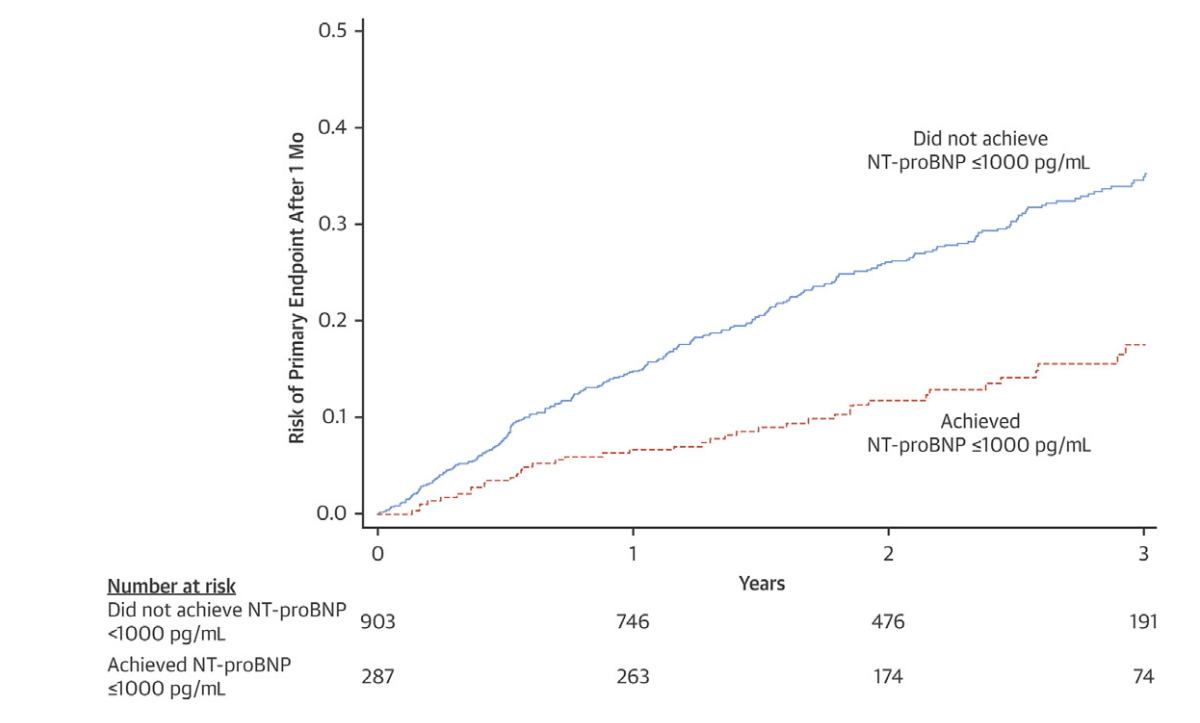
\includegraphics{../../images/NTBNP_zile.png}   \caption{Risk of primary endpoint after 1 month of randomization in patients with a baseline amino terminal pro B-type natriuretic peptide (NT proBNP) of greater than 1000 pg/mL. The risk at 3 years of follow-up was 50\% less in those who achieved an NT-proBNP of less than 1000 pg/mL than in those who did not. \citep{Zile2016}}   \label{NTBNP_zile} \end{figure} %PROGNOSIS

The associations between plasma BNPs and prognosis has provided the rationale for a series of controlled trials of hormone-guided therapy in chronic HF. Although individual trials have variously yielded positive or neutral results, serial meta-analyses have consistently indicated benefit from guided therapy with greater than 20\% reductions in total mortality and HF hospitalizations. Metaanalyses of trials of NTproBNP–guided therapy in chronic heart failure suggest improved outcomes and confirm achievement of NTproBNP of less than 1000 pg/mL confers a better prognosis. All trials of marker-guided therapy have consistently confirmed the strong association between achieved plasma B-type  peptide levels and outcome regardless of allocated treatment strategy. \citep{Troughton2014} %TREATMENT

\begin{figure}   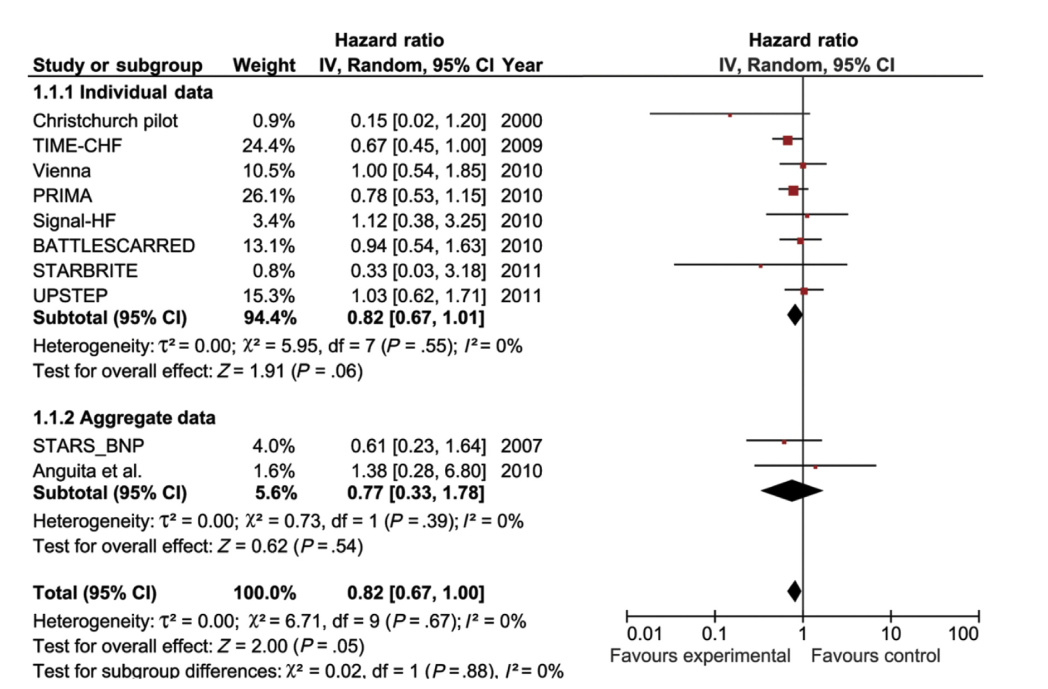
\includegraphics{../../images/NP_treatment.png}   \caption{Forest plot of mortality among participants in trials of marker-guided treatment of chronic heart failure showing unadjusted individual and mean hazards ratios with 95\% confidence intervals (CIs) for 8 studies providing individual patient data and 2 studies providing aggregate data. \citep{Troughton2014}}   \label{NP_treatment} \end{figure} %TREATMENT

Risk calculators would likely be improved by incorporation of markers such as NT-proBNP. May and colleagues assessed the performance of the Seattle Heart Failure Model in ambulant chronic heart failure and found, in a subgroup of 544 out of 4077 registered patients with BNP results available, that the marker modestly augmented the c-statistic for prediction of the composite endpoint of survival free from death, transplantation, or LV assist device implantation from 0.73 to 0.78 for events at 1 year. \citep{May2007} %PROGNOSIS

Subsequent studies were aimed at discovering family members which resulted in the isolation of two other factors which were named brain natriuretic peptide (BNP) and C-type natriuretic peptide (CNP). Studies also showed that although BNP was first isolated from the brain, that it is predominantly expressed in the ventricle. ANP and BNP were therefore renamed A-type and B-type natriuretic peptide, respectively, to better reflect their position in the family and to also lessen the misleading nature of the nomenclature of BNP as a cardiovascular and not a neural factor. ANP and BNP are the natriuretic peptides which are expressed predominantly in the atria and ventricle, respectively, and are referred to as the cardiac natriuretic peptides. CNP is differentially expressed mainly in the nervous system and vasculature (e.g. endothelial cells, monocyte / macrophages) and is involved mainly in neural regulation as well as vascular control although its role is still unclear. \citep{Suzuki2001} %PHYSIOLOGY%

Other NPs that share a common biochemical structural feature, a 17-amino-acid ring and a disulfide bridge between cysteine molecules, have been discovered since: urodilantin (an isoform of ANP), C-type natriuretic peptide, and Dendroaspis natriuretic peptide. \citep{Gaggin2014} %PHYSIOLOGY%

Each natriuretic peptide is coded by a separate gene but shows similar exon--intron properties. In humans, the ANP and BNP genes are located 8 kilobases apart on chromosome 1 and the CNP gene is located on chromosome 2. Each natriuretic peptide gene produces a prohormone or precursor protein. ANP is synthesized as a 126 amino acid precursor protein which is cleaved to produce a 96 amino acid amino-terminal fragment and a 28 amino acid carboxyl-terminal fragment. The carboxyl-terminal 28 amino acid fragment is the biologically active peptide and has a shorter half-life than the amino-terminal fragment. Similarly, BNP is produced as a 108 amino acid precursor protein which is cleaved into a biologically active 32 amino acid carboxyl-terminal fragment and a 76 amino acid amino-terminal fragment. CNP produces 22 and 53 amino acid fragments. The 22 amino acid fragment is the mature and more active form, and is expressed in the nervous system and endothelial cells. The common property of the natriuretic peptides is the formation of a disulfide bond which results in a ringed structure (Fig. 1).\citep{Suzuki2001} %PHYSIOLOGY%

ANP is encoded by the NPAA gene on chromosome 1. It is translated into a 151-amino-acid pre-prohormone (preproANP) that is cleaved in the sarcoplasmic reticulum to a 126-amino-acid prohormone (proANP), which is stored in intracellular granules.  When stimulated and released, proANP is further cleaved into a 28-amino-acid bioactive form (ANP) and a 98-amino-acid N-terminal fragment (NT-proANP). The half-life of ANP is approximately 2 minutes, whereas NT-proANP half-life is variable depending on the fragment measured. \citep{Volpe2016} %\citep{Maisel2018} %PHYSIOLOGY%

ANP is predominanlty produced in the atria of the heart and to a lesser extent the ventriclesn and extracardiac tissues, such as the kidney.  Unlike BNP, which has minimal preformed and  stored hormone, most proANP is stored in intracellular granules of the atria and released on stimulation, whereas further production of ANP involves the slower process of transcription and translation.  The major stimulus for ANP release is increased atrial wall stretch reflecting increased intravascular volume.  Other stimuli for release include catecholamines, arginine vasopressin, and endothelin.  These stimuli reflect the counter-regulatory role ANP plays against volume overload and hypertension.  \citep{Maisel2018} %PHYSIOLOGY%

BNP was first described in 1988 after isolation from porcine brain tissues (hence its original name brain natriuretic peptide) with subsequent studies finding it produced in the cardiac ventricles.  As with ANP, BNP is a peptide neurohormone synthesized by vardiac ventricular myocytes in response to mechanical stretch.  During periods of volume overload, mechanical stretch on cardiomyocytes membranes activates signal transduction leading to downstream transcription and translation or preproBNP, a 134 amicoacid precursor peptide. \citep{Maisel2018} %PHYSIOLOGY%

PreproBNP undergoes a 2-step enzymatic cleavage to produce the biologically active product.  The first cleavage occurs in the sarcoplasmic reticulum during RNA translation, removing a 26-amino-acid signaling peptide and producing proBNP.  proBNP subsequently undergoes a second cleavage by prohormone convertases (including corin and furin) to produce the biologically active C-terminal peptide, BNP, and an inactive N-terminal fragment, NT-proBNP.  \citep{Hammerer-Lercher2008} %\citep{Maisel2018} %PHYSIOLOGY%

BNP and NT-proBNP are secreted in equimolar quantites into the circulation.  BNP has a serum half-life of 20 minutes, whereas NT-proBNP has a half-life of 120 minutes. \ref{NP_physiology} \citep{DanielsandMaisel2007} %\citep{Maisel2018} %PHYSIOLOGY%

\begin{figure}

    \centering

    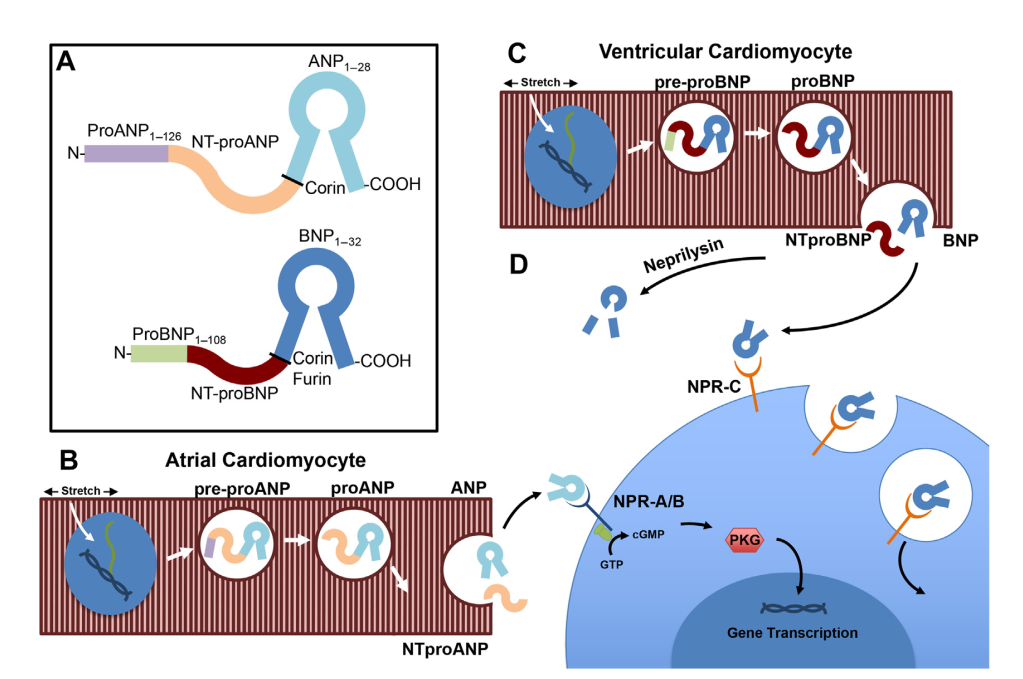
\includegraphics[scale=0.4]{../../images/NP_physiology.png}

    \caption{ANP and BNP physiology. (A) Molecular structure of ANP (top) and BNP (bottom) showing enzymatic cleavage sites and end-product fragments. (B) Production and processing of ANP by atrial cardiac myocyte in response to mechanical stretch stimulus. (C) Production and processing of BNP by ventricular cardiac myocyte in response to mechanical stimulus. (D) Effects of ANP and BNP on target tissues. Both ANP and BNP bind NP receptor (NPR)A and NPR-B on target cells, inducing cleavage of guanosine triphosphate (GTP) to cyclic guanosine monophosphate (cGMP) by cytoplasmic G proteins, initiating an intracellular cGMP signaling cascade involving protein ki- nase G (PKG), ultimately leading to downstream transcription of genes involving smooth muscle cell relaxation, diuresis and natriuresis (depending on target tissue). Both ANP and BNP are broken down in serum by circulating endogenous peptidases, including neprilysin. ANP and BNP are also degraded (to a lesser extent) by cellular uptake through binding NPR-C, undergoing receptor-mediated endocytosis and intracellular breakdown by lysosomes. \citep{Maisel2018}}

    \label{NP_physiology}

\end{figure}

ANP and BNP interact with 3 NP receptors (NPRS; A,B and C)  with their main physiologic effects exerted through the NPR-A receptor.  The NPR-A is the predominant form on the blood vessels, with a smaller amount of NPR-B, and both receptors are found in the kidneys and adrenal glands.  ANP and BNP binding to NPR-A and NPR-B leads to activation of guanylyl cyclase and downstream signaling through cyclic guanosine monophgosphate (cGMP).  NPR-C clears ANP, and to a lesser extent, BNP by binding and internalizing the receptor and degrading the hormone.  ANP is also inactivated and cleared by neutral endopepitdases NEPs. \ref{NP_physiology} \citep{Maisel2018}  %PHYSIOLOGY%

ANP signaling leads to a reduction in blood pressure, natriuresis, and diuresis. These actions are predominantly performed via effects on the kidneys. ANP increases renal blood flow, dilates afferent arterioles, and constricts efferent arterioles, leading to increased glomerular filtration. 16 It inhibits angiotensin II–mediated sodium and water reabsorption in the proximal tubule, inhibits sodium reabsorption in the inner medullary ducts, and antagonizes vasopressin, leading to decreased water reabsorption in the collecting duct. These effects lead to apotent diuresis and natriuresis. Outside of the kidney, ANP reduces blood pressure by decreasing sympathetic output, increasing venous capacitance, and increasing vascular permeability. These actions seem to be mediated by ANP inhibiting catecholamines, renin, angiotensin II, aldosterone, and endothelin. ANP also directly affects the heart, preventing hypertrophy. \citep{Maisel2018} %PYSIOLOGY%

When BNP circulates and binds NPRs on target tissues, it triggers increased intracellular cGMP signaling cascades, inducing actions that reduce cardiac preload and afterload to counteract the detrimental effects of pressure and volume overload, as seen in HF. BNP is primarily cleared through degradation by circulating neutral endopeptidases and, to a lesser extent, through uptake by NPR-C in peripheral tissues and minimally through renal excretion (see Fig. \ref{NP_physiology}). These physiologic processes are counter-regulatory to the detrimental neurohormonal activation of the sympathetic nervous system and RAAS in HF and are why ANP and BNP levels reflect HF severity. \citep{Potter2011} %\citep{Maisel2018}  %PHYSIOLOGY%

Although the molecular structure and cellular production of BNP was first described in the late 1980s, its clinical significance was not fully elucidated until the early 2000s. The evidence is now overwhelming that early measurement of serum BNP levels should be used to diagnose acute heart failure (AHF), and it is a class I indication in the American Heart Association (AHA)/American College of Cardiology (ACC) guidelines for the management of HF that BNP levels should be measured in all hospital admissions for AHF. Cardiac-specific biomarkers are particularly useful in the emergency department (ED) setting when evaluating dyspneic patients, because it is difficult to distinguish between shortness of breath caused by HF versus that caused by pulmonary disease. \citep{Maisel2018} %DIAGNOSIS%

The Breathing Not Properly Multinational Study published in 2002 was the first large study to evaluate the efficacy of BNP as a cardiac biomarker for diagnosis of HF in the ED setting. This study evaluated 1586 patients presenting to EDs with the chief complaint of dyspnea at different medical centers around the world. Serum BNP levels were higher in patients presenting with dyspnea caused by AHF than in dyspnea from a noncardiac cause. Serum BNP levels were positively correlated with severity of HF using the New York Heart Association (NYHA) classification. Using a BNP cutoff of 100 pg/mL, serum BNP level was 90\% sensitive and 76\% specific for HF. Using a cutoff of 50 pg/mL, BNP had a negative predictive value of 96\%. \citep{Maisel2002} %\citep{Maisel2018} %DIAGNOSIS%

The Pro-BNP Investigation of Acute Dyspnea in the Emergency Department (PRIDE) study published similar findings using NT-proBNP in 2005. NT-proBNP level was highly sensitive and specific at diagnosing AHF among 600 patients presenting to the ED with dyspnea using a cutoff level of 300 pg/mL, and NT-proBNP was 90\% sensitive and 85\% specific for diagnosis of AHF. \citep{Januzzi2005}  %\citep{Maisel2018} %DIAGNOSIS%

Because of the speed and ease of measuring serum biomarkers, use of BNP in EDs has the potential to greatly reduce hospital stay and overall treatment costs associated with HF. \citep{Mueller2004} evaluated 452 patients presenting to the ED with acute dyspnea and found that measurement of BNP led to more rapid HF diagnosis, which reduced time to discharge and decreased overall cost of treatment associated with the ED visit.  %\citep{Maisel2018} %DIAGNOSIS%

The Canadian Multicenter Improved Management of Patients With Congestive Heart Failure (IMPROVE-CHF) study showed similar findings using NT-proBNP in a population of 500 patients presenting to 7 different EDs in Canada. Measurement of serum NT-proBNP level to aid in the diagnosis of HF reduced duration of ED visits by 21\%, reduced the rate of rehospitalization after 60 days by 45\%, and similarly reduced the overall cost of treatment of these patients. \citep{Moe2007} %\citep{Maisel2018} %DIAGNOSIS%

In 2002, Berger and colleagues  evaluated 452 ambulatory patients to determine whether serum BNP levels were predictive of future sudden cardiac death (SCD) in patients with a left ventricular ejection fraction (LVEF) less than 35\% within a 3-year follow-up period. Patients with a baseline serum BNP level greater than 130 pg/mL had higher rates of SCD, and the investigators suggested that patients with an increased BNP level at baseline should be evaluated for implantable cardiac defibrillator therapy. \citep{Berger2002} %\citep{Maisel2018} %PROGNOSIS%

A substudy of the A Randomized Trial of the Angiotensin-Receptor Blocker Valsartan in Chronic Heart Failure (Val-HeFT) trial also evaluated the prognostic value of BNP. This analysis was of 4300 patients who had serial serum BNP levels drawn at baseline, 4 months, and 12 months after enrollment. Patients with the largest percentage decline in BNP level from baseline during follow-up had the lowest morbidity and mortality. In contrast, patients with the highest percentage increase in BNP from baseline had the worst morbidity and mortality using a Cox proportional hazard model. \citep{Anand2003} %\citep{Maisel2018} %PROGNOSIS%

The 2004 Rapid Emergency Department Heart Failure Outpatients Trial (REDHOT) trial evaluated 464 patients presenting to the ED with dyspnea and with NYHA class II to IV HF with baseline BNP greater than 100 pg mL. The investigators found that baseline BNP levels greater than 200 pg/mL were strongly predictive of 90-day outcomes (combined HF visits, admissions, and mortality). \citep{Maisel2004} %\citep{Maisel2018} %PROGNOSIS%

An analysis of the PRIDE trial examined 1-year outcomes of patients presenting to the ED with acute dyspnea. NT-proBNP levels greater than 986 pg/mL at baseline were associated with more severe HF, and a single baseline NT-proBNP level increased above this cutoff was the strongest individual predictor of death at 1 year. \citep{Januzzi2006b} %\citep{Maisel2018} %PROGNOSIS%

Failure of NP levels to decrease during an HF hospitalization while undergoing treatment is associated with worse prognosis and suggests a potential role for serial BNP measurement during HF hospitalization. \citep{Cheng2001} evaluated 72 male veterans admitted with decompensated NYHA class III to IV HF and followed them for 30 days after discharge. Serial BNP levels were followed, starting with baseline values drawn within 24 hours of admission. Of these patients, 13 died and 9 were readmitted during the study period. Patients who died or were readmitted had increasing BNP levels during hospitalization. Patients who survived and were not readmitted showed decreasing BNP levels during admission. \citep{Cheng2001} %\citep{Maisel2018} %PROGNOSIS%

In a study of 50 patients admitted for AHF, \citep{Bettencourt2002} measured BNP levels at admission and then serially throughout hospitalization. Patients were followed for 6 months after discharge to determine whether BNP trends during the index hospitalization were predictive of end points including readmission for cardiovascular causes and death. Patients who died or were readmitted had less marked decline in BNP levels during hospitalization (770 \pm 608 pg/mL to 643 \pm 465 pg/mL; P=0.08), whereas increasing BNP levels during hospitalization were associated with increased event rate (hazard ratio=3.3; 95\% confidence interval, 1.3–8.8). %\citep{Maisel2018} %PROGNOSIS%

In the Acute Decompensated Heart Failure National Registry (ADHERE) database of 65,275 patients with AHF, increased serum BNP levels at time of admission for HF exacerbation correlated with an increased risk of in-hospital mortality. \citep{Fonarow2007} %\citep{Maisel2018} %PROGNOSIS%

In a study of the Get With the Guidelines Heart Failure Registry, 99,930 patients with AHF were stratified into subgroups based on gender and LVEF (reduced, $<$ 40\%; borderline, 40\%–49\%; preserved, $\geq$ 50\%). Regardless of gender or LVEF, patients with BNP levels greater than the median had a higher mortality than those less than the median serum BNP level. \citep{Hsich2013}  %\citep{Maisel2018} %PROGNOSIS%

A substudy of the Framingham Offspring Study evaluated 3346 asymptomatic patients in the ambulatory setting and measured their serum BNP values over time. An increased BNP level greater than the 80th percentile was associated with an increased risk of death, first major cardio- vascular event, atrial fibrillation (AF), stroke or transient ischemic attack, and HF. \citep{Wang2004c} %\citep{Maisel2018}  %PROGNOSIS%

\citep{Kazanegra2001} measured serial serum BNP levels and pulmonary capillary wedge pressures using Swan-Ganz catheters in patients admitted to the hospital for an AHF exacerbation. Treatment-related decreases in pulmonary capillary wedge pressures corresponded with declining serum BNP levels, suggesting that BNP levels should decline with diuresis. %\citep{Maisel2018} %TREATMENT%

The Plasma Brain Natriuretic Peptide-Guided Therapy to Improve Outcome in Heart Failure (STARS-BNP) trial published in 2007 evaluated the use of BNP-guided treatment strategies compared with standard clinical therapy in 220 patients with NYHA class II to III HF who were taking optimal medical management (angiotensin-converting enzyme [ACE] inhibitors, b-blockers, and diuretics). Patients were randomized to receive BNP-guided treatment with a goal BNP level of less than 100 pg/mL or treatment guided by clinical and symptomatic improvement. By 15-month follow-up, patients in the BNP-guided treatment arm had a significantly lower primary outcome of HF-related death or readmission (24\% vs 52\%; P$<$.001). \citep{Jourdain2007} %\citep{Maisel2018} %TREATMENT%

The 2009 NT-proBNP–Assisted Treatment To Lessen Serial Cardiac Readmissions and Death (BATTLESCARRED) trial found similar results using NT-proBNP–guided clinical management. In this trial, 364 patients admitted for HF exacerbation were assigned to NT-proBNP guided therapy, intensive clinical management (using aggressive uptitration of HF medications to optimal clinical trial doses), or usual care using symptom-guided management. At 1-year follow-up, mortality was significantly lower in the NT-proBNP guided treatment arm versus usual care (9.1\% vs 18.9\%; P=.03). By 3-year follow-up, mortality was significantly lower in the NT-proBNP guided group (15.5\%) compared with the intensive clinical management group (30.9\%; P=0.048) and usual care group (31.3\%; P=0.021). \citep{Lainchbury2009} %\citep{Maisel2018} %TREATMENT%

The 2009 Trial of Intensified versus Standard Medical Therapy in Elderly Patients With Congestive Heart Failure (TIME-CHF) study also evaluated NT-proBNP–guided therapy.This trial included 499 patients with chronic HF who were older than 60 years, NYHA class greater than II, hospitalized for HF within the last year, and had a baseline NT-proBNP level greater than twice the upper limit of normal. These patients were followed for 18 months after initial admission, and the NT-proBNP–guided therapy arm had higher rates of survival and lower rates of all-cause hospitalizations in patients aged 60 to 75 years but not in patients older than 75 years (P<.02). \citep{Pfisterer2009} %\citep{Maisel2018} %TREATMENT%

In addition, a 2014 meta-analysis by Troughton and colleagues 71 evaluated BNP-guided treatment in 2000 patients with HF and confirmed that BNP-guided treatment reduced all-cause mortality in patients less than 75 years old. BNP-guided treatment reduced hospitalizations caused by HF and cardiovascular disorders in all patients regardless of age or LVEF. \citep{Troughton2014} %\citep{Maisel2018} %TREATMENT%

Higher baseline levels of BNP have been observed with increasing age; however, the exact mechanism is unknown. This age-related increase was independent of age-related diastolic dysfunction. Some investigators have hypothesized that this is caused by reduced expression of NPRs with age, which could result in decreased clearance of circulating BNPs in older patients. \citep{Maisel2018} %LIMITATIONS%

Several studies have shown that women have higher levels of BNP and NT-proBNP. These studies evaluated age matched cohorts in which serum BNP and NT-proBNP levels were higher in women than in men at any age, although the reason for this finding was not clear. Some have proposed that estrogen levels may play a role in this observation, because women on hormone replacement therapy had higher baseline serum BNP levels than those not taking hormone therapy. \citep{Maisel2018} %LIMITATIONS%

Renal dysfunction may cause increases in baseline serum NP levels, but the reason for this is not clearly understood. BNP is primarily cleared from circulation through degradation by circulating endogenous peptidases rather than by renal clearance. The mechanism behind this observation is probably multifactorial, considering that patients with renal dysfunction tend to be older and less healthy, with higher intravascular volume and ventricular strain contributing to increased baseline BNP levels independently of renal function. \citep{Maisel2018} %LIMITATIONS%

Although obesity is a well-documented factor that can decrease baseline serum BNP level, the exact mechanism behind this remains unclear.  Adipocytes are known to have increased concentration of NPRs, thus obese patients may have greater clearance of BNP by adipocytes. However, other studies have shown a correlation between BNP levels and lean mass rather than fat, which contradicts this hypothesis.  It is less clear whether serum NT-proBNP level is similarly decreased in obese patients, and, unlike BNP, NT-proBNP is not cleared by NPRs (natriuretic peptide receptors). \citep{Maisel2018} %LIMITATIONS%

The 2014 Angiotensin–Neprilysin Inhibition versus Enalapril in Heart Failure (PARADIGM-HF) trial compared the novel neprilysin-angiotensin inhibitor LCZ696, a combination of the salt form of valsartan combined with sacubitril (an inhibitor of neprilysin, a circulating neutral endopeptidase involved in the degradation of NPs), with the ACE inhibitor enalapril and showed a dramatic improvement in the primary outcome of mortality and HF hospitalization with LCZ696. \citep{McMurray2014} %\citep{Maisel2018} %\citep{Maisel2018} %TREATMENT%

As the clinical use of sacubitril-valsartan becomes more widespread, there is a growing concern that the measurement of serum NP levels in patients taking this drug may be problematic. In patients taking the neprilysin inhibitor, levels of BNP, which is broken down by neprilysin among other enzymes, may be increased because of decreased serum breakdown rather than because of change in underlying disease state (such as volume overload in AHF), potentially interfering with the prognostic and diagnostic utility of BNP.  \citep{Mckie2016} %\citep{Maisel2018} %LIMITATIONS%

Results from the PARADIGM-HF trial did show that plasma BNP concentrations were significantly increased in patients taking sacubitril-valsartan versus enalapril, whereas NT-proBNP levels were significantly lower in the sacubitril-valsartan group.  However, the decreases were only modest and, although significantly different between the two treatment arms, the mean serum values in each group decreased to well within the anticipated variation of these biomarkers.  Neprilysin primarily breaks down ANP and CNP, whereas BNP may be more resistant to neprilysin cleavage.  As such, serum BNP levels may be less affected by neprilysin inhibition, as implied by initial interpretations of the PARADIGM-HF trial results. \citep{Maisel2018} %LIMITATIONS%

Although more studies will be needed to determine the exact effect of neprilysin inhibition on BNP, there are some data to support that NT-proBNP may be more reliable in patients taking sacubitril.  The earlier Angiotensin Receptor Neprilysin Inhibitor LCZ696 in Heart Failure with Preserved Ejection Fraction (PARAMOUNT) trial examined effects of sacubitril-valsartan compared with valsartan alone in patients with chronic HF with preserved ejection fraction. Although significant early declines in NT-proBNP were observed at 12 weeks, NT-proBNP levels were no longer significantly different between the two groups after 36 weeks. Serum BNP was not measured in this trial.  \citep{Maisel2018} %LIMITATIONS%

The biological actions of natriuretic peptides are mediated through membrane-bound natriuretic peptide receptors (NPR) that are linked to a cyclic guanosine monophosphate-dependent signaling cascade, including NPR-A, which preferentially binds ANP and BNP, and NPR-B, which preferentially binds CNP. %PHYSIOLOGY%



Elevated natriuretic peptides levels can be found in many circumstances involving LV dysfunction or hypertrophy; right ventricular (RV) dysfunction secondary to pulmonary diseases; cardiac inflammatory or infectious diseases; and endocrinologic diseases and high output status without decreased left ventricular ejection fraction (EF), e.g., sepsis, renal failure, cirrhosis of liver, or intracranial pathologies. The causes and mechanisms of elevated natiuretic peptides levels are summarized in Fig. \ref{NP_causes}. %The potential clinical applications in the non-HF settings are summarized in Table \ref{NP_applications}. %PHYSIOLOGY%



\begin{figure}

    \centering

    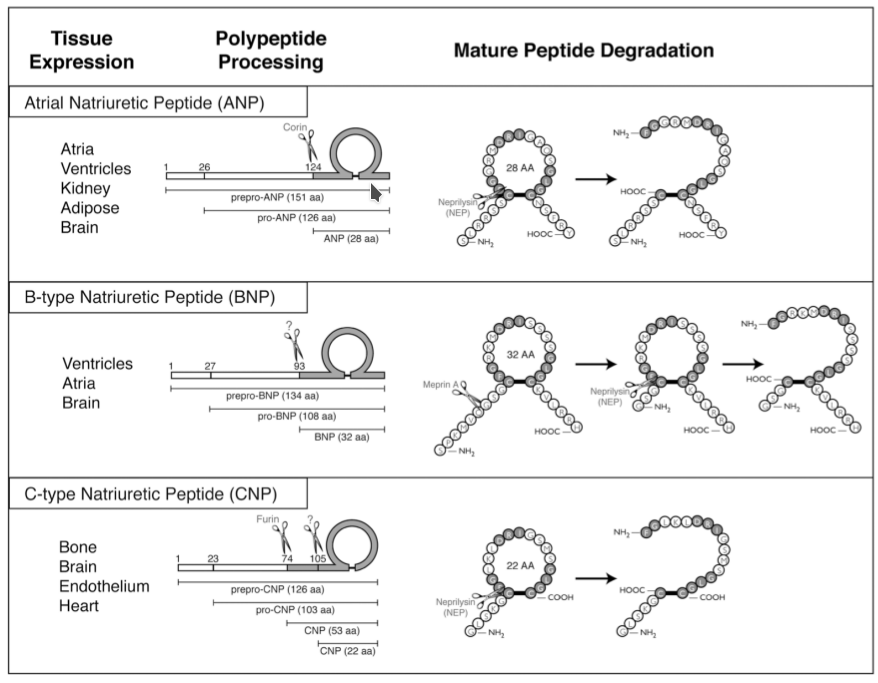
\includegraphics[scale=0.4]{../../images/NP_structure.png}

    \caption{Structure of the human natriuretic peptides. The structure of the preprohormones for ANP, BNP and CNP are outlined on the left of each panel. The final amino acid sequence and structure of the mature peptides along with the major degradation product are shown on the right. The sites of cleavage are indicated with scissors.}

    \label{NP_structure}

\end{figure}



\subsubsection{Atrial Natriuretic Peptide}



All natriuretic peptides are synthesized as preprohormones Fig \ref{NP_structure}. %PHYSIOLOGY%

The resulting mRNA gives rise to a 151 amino acid polypeptide, known as preproANP. The first 25 amino acids constitute a signal sequence that is cleaved to yield a 126 amino acid peptide called proANP, which is the major form of ANP stored in the atrial granules. %PHYSIOLOGY%

Upon release from these granules, proANP is rapidly cleaved by corin, a transmembrane cardiac serine protease. Corin is highly expressed on the extracellular surface of atrial cardiomyocytes and cleaves proANP into the biologically active 28-amino acid form of ANP \citep{Yan2000}. %PHYSIOLOGY%

Mice lacking functional corin have dramatically reduced levels of fully processed ANP in their hearts and are mildly hypertensive \citep{Chan2005}. %PHYSIOLOGY%

Alternative processing of proANP in the kidney by an unknown protease results in a 32-amino acid peptide called urodilatin that contains four additional amino-terminal residues. %PHYSIOLOGY%

Release of proANP from the atrial granules is primarily stimulated by stretch of the atrial wall caused by increased intravascular volume, but pressor hormones also stimulate ANP release \citep{Ruskoaho2003}. %PHYSIOLOGY%



ANP is secreted in response to:

    \begin{itemize}

        \item Stretching of the atrial wall \citep{Widmaier2008}

        \item Reduced Sympathetic stimulation of $\beta$-adrenoceptors

        \item Raised sodium concentration (hypernatremia), though sodium concentration is not the direct stimulus for increased ANP secretion. \citep{Widmaier2008}

        \item Endothelin, a potent vasoconstrictor

        \item exercise \citep{Kokkonen2002}

    \end{itemize}





\begin{figure}

    \centering

    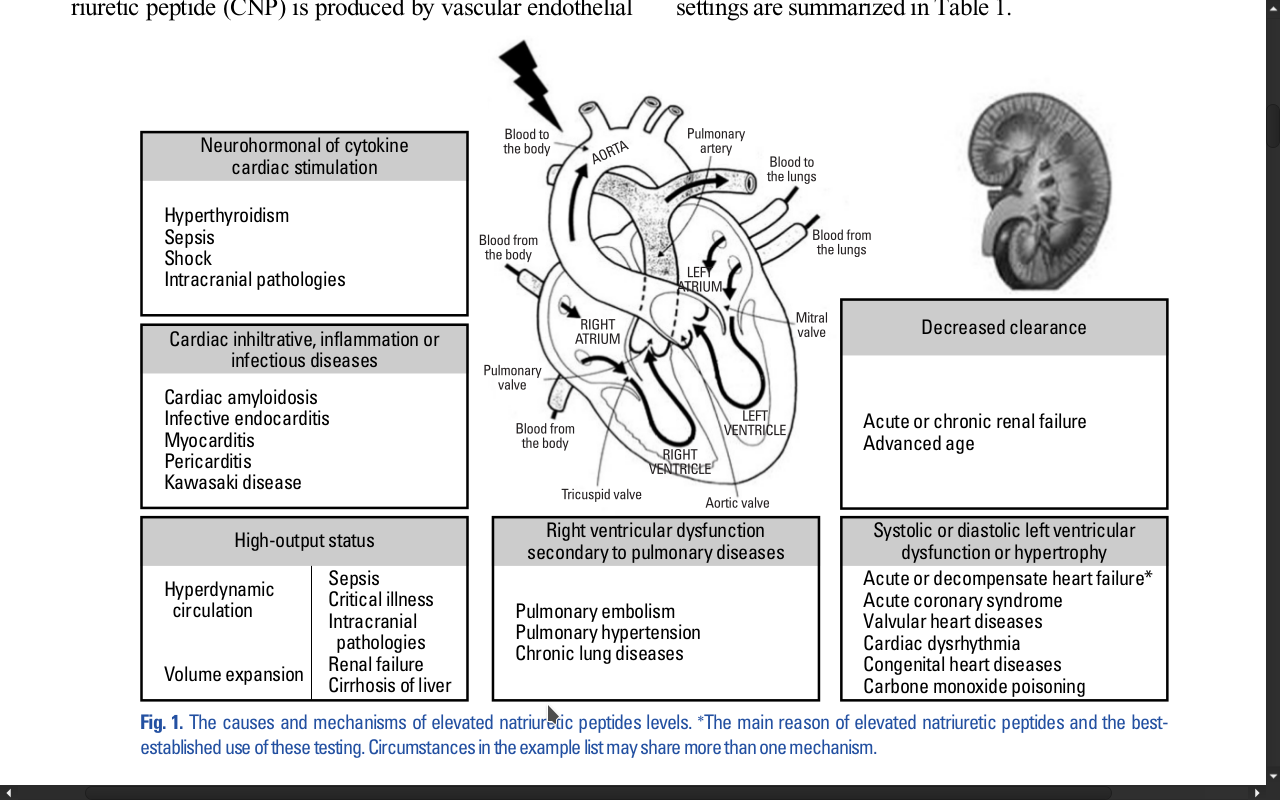
\includegraphics[scale=0.3]{../../images/NP_causes.png}

    \small\caption{The causes and mechanisms of elevated natriuretic peptides levels.}

    \label{NP_causes}

\end{figure}



% \begin{table}

%     \centering

%     \caption{Potential Clinical Applications of Natriuretic Peptides in Selected Diseases}

%     \begin{tabular}{|l|c|c|c|}

%         \hline

%         Diseases & Screening \footnote{Screening for the presence of cardiac dysfunction} &  & Prognosis \\

%         \hline

%         Heart failure \footnote{The best-established clinical application of these natriuretic peptides testing} & + & + & + \\

%         Acute coronary syndrome & + & + & + \\

%         Cardiac procedures & + & + & + \\

%         Pulmonary embolism & + & + & + \\

%         Pulmonary hypertension & + & + & - \\

%         Chronic lung diseases & + & + & + \\

%         Valvular heart diseases & + & + & N/A \\

%         Cardiac dysrhythmia & + & + & +/- \\

%         Cardiac inflammatory or infectious diseases & + & + & N/A \\

%         Cardiogenic syncope & + & N/A & N/A \\

%         Sleep apnea & + & + & N/A \\

%         Hypertension & + & + & N/A \\

%         Sepsis & + & + & + \\

%         Renal failure & + & + & + \\

%         Cirrhosis of liver & + & + & + \\

%         Hyperthyroidism & + & + & N/A \\

%         Intracranial pathologies & + & + & + \\

%         Epilepsy / Seizures & + & - & - \\

%         Carbone monoxide poisoning & + & N/A & N/A \\

%         \hline

%     \end{tabular}

%     \label{NP_applications}

% \end{table}



\subsubsection{B-Type Natriuretic Peptide}



BNP can be produced in both atria and ventricles, and is upregulated in failing ventricular myocardium. In response to increased myocardial stretch and wall stress, ventricular myocytes secret the pro-hormone pre-proBNP, which is then cleaved into biologically active BNP and the inactive byproduct N-terminal-proBNP (NT-proBNP). Elevated BNP levels have been demonstrated to be a response to increased angiotensin II and sympathetic tones. \citep{Iwanaga2006} %PHYSIOLOGY%





BNP is eliminated by binding to the NPR-C or degradation by NEP on endothelial cells, smooth muscle cells, cardiac myocytes, renal epithelium, and fibroblasts. NT-proBNP is cleared mainly by the kidney. Compared to ANP, circulating BNP has a significantly longer half-life of around 20 min in humans; the half-life of NT-proBNP is about 60-90 minutes and would be expected to be longer in the setting of renal dysfunction. Unlike ANP, BNP is not initially cleaved by NEP. Instead, the first six amino-terminal amino acids of BNP are first cleaved by the metalloprotease, meprin A in the kidney brush border, which then allows further degradation by NEP \citep{Pankow2007}. Obese patients tend to have lower BNP levels than others. Neural endopeptidases that can be secreted by adipose tissue may be related to increased BNP clearance in obese patients.\citep{Yang2004} %PHYSIOLOGY%



Plastic tubes containing ethylenedinitrolotetraacetic acid (EDTA) are desirable for BNP determination and refrigeration is required if the interval between blood collection and analysis is over 4 hours; whereas NT-proBNP can be measured in both serum or plasma, collected in glass or plastic tubes, and has no significant loss of immunoreactivity after 48 hours at room temperature. \citep{Omland2008} %PHYSIOLOGY%



\subsubsection{C-Type Natriuretic Peptide}

C-type natriuretic peptide (CNP) was initially purified and sequenced from porcine brain extracts. It is the most highly expressed natriuretic peptide in the brain but is also highly expressed in chondrocytes and endothelial cells. Unlike ANP and BNP, the human gene encoding CNP, NPPC, is not located on chromosome 1 but on chromosome 2. %PHYSIOLOGY%



Processing of proCNP to its mature form may occur through the action of the intracellular serine endoprotease, furin. In vitro, furin cleaves the 103 amino acid proCNP into a 53 amino acid carboxyl-terminal biologically active peptide \citep{Wu2003a}. This 53 amino acid form of CNP (CNP-53) is the major active form of CNP, at the tissue level. However, in the systemic circulation, a shorter 22 amino acid form dominates (CNP-22). The protease responsible for this cleavage is not known. Importantly, CNP-53 and CNP-22 appear to bind and activate their cognate receptor, NPR-B, equally well. %PHYSIOLOGY%



CNP is not stored in granules and its secretion is increased by growth factors and sheer stress in cultured endothelial cells. CNP expression in neo-intimal vascular smooth muscle cells is increased in response to vascular injury. In normal human subjects, mean CNP concentration is very low (1 fmol/ml). It is elevated in patients with congestive heart failure, although to a much lower extent than ANP and BNP \citep{Charles2006} \citep{Del-Ry2005} \citep{Kalra2003}. %PHYSIOLOGY%



\subsection{Natriuretic Peptide Receptors}

There are three known natriuretic peptide binding proteins. All members contain a relatively large (\\~450 amino acid) extracellular ligand binding domain and a single membrane-spanning region of about 20 residues. Natriuretic peptide receptors A and B contain an equally large intracellular domain consisting of a so-called kinase homology domain, dimerization domain, and carboxyl-terminal guanylyl cyclase domain. Thus, NPR-A and NPR-B signal by catalyzing the synthesis of the intracellular signaling molecule cGMP. In contrast, NPR-C only contains a 37 residue intracellular domain and lacks guanylyl cyclase activity. It primarily controls local natriuretic peptide concentrations via receptor-mediated internalization and degradation \citep{Rose2008}. %PHYSIOLOGY%



\begin{figure}

    \centering

    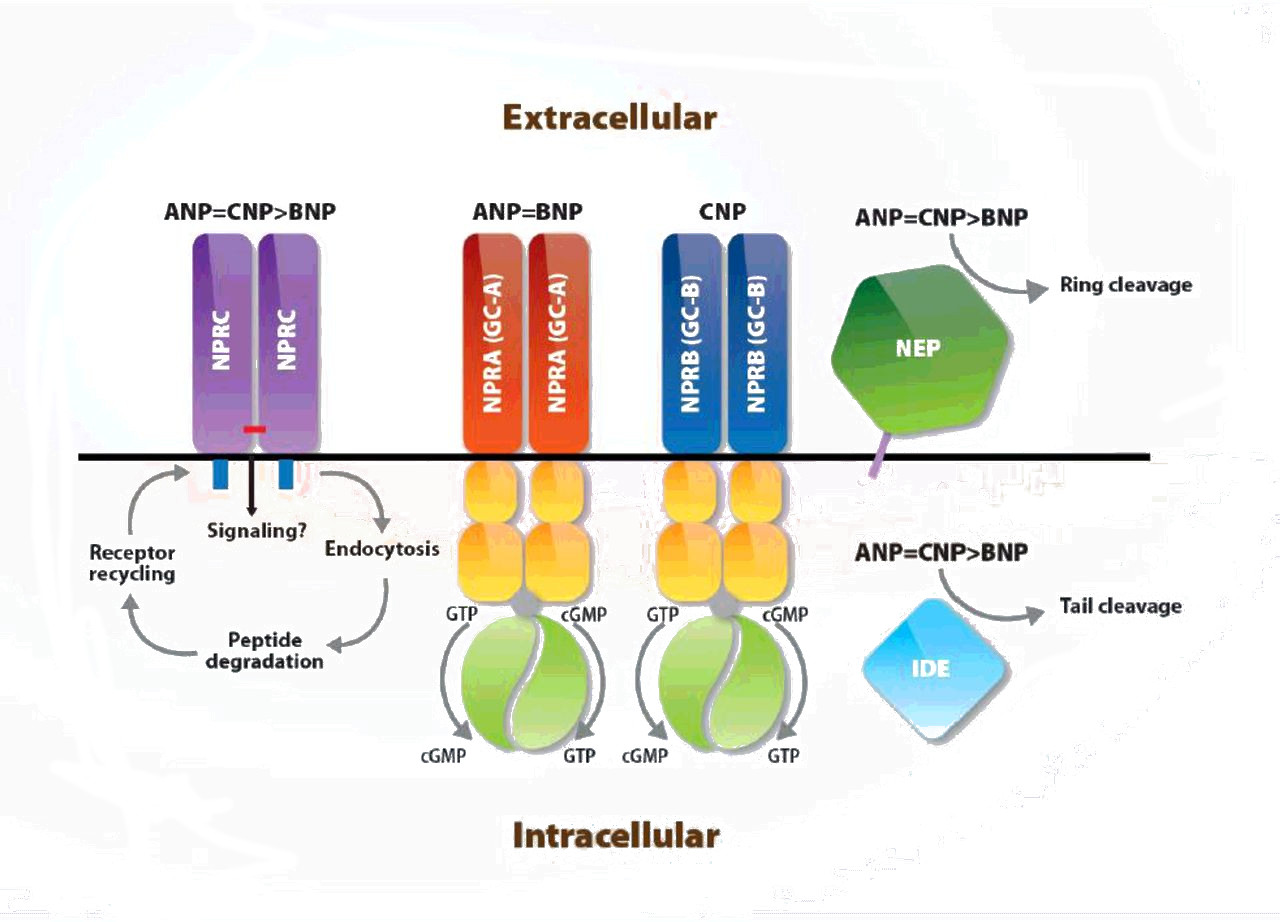
\includegraphics[scale=1]{../../images/NP_receptors.jpg}

    \small\caption{Schematic representation of natriuretic receptors}

    \label{NP_receptors}

\end{figure}





\subsubsection{Natriuretic Peptide Receptor-A}



NPR-A internalization and degradation is also controversial. One group consistently reports that the majority of internalized ANP-NPR-A complexes are degraded via a lysosomal pathway with a small portion returning intact to the plasma membrane \citep{Pandey2002}. Meanwhile, studies in primary kidney and Chinese Hamster ovary indicate that NPR-A is a membrane resident protein that does not undergo acute internalization and degradation \citep{Fan2005} \citep{Vieira2001}. %PHYSIOLOGY%



NPR-A and/or its mRNA is expressed in kidney, lung, adipose, adrenal, brain, heart, testis, and vascular smooth muscle tissue \citep{Goy2001}. NPR-A null mice exhibit chronic salt-resistant hypertension and cardiac hypertrophy and fibrosis \citep{Kuhn2002}.  A deletion in the human NPR-A gene was identified in nine Japanese individuals, of which eight had essential hypertension; the normotensive individual with the altered allele had left ventricular hypertrophy \citep{Nakayama2000}. %PHYSIOLOGY%



\subsubsection{Natriuretic Peptide Receptor-B}



NPR-B dephosphorylation has been shown to mediate desensitization in response to prolonged CNP exposure, protein kinase C activation, and intracellular calcium elevations \citep{Potter2000} \citep{Potthast2004}. NPR-B and/or its mRNA is expressed in bone, brain, fibroblasts, heart, kidney, liver, lung, uterine, and vascular smooth muscle tissue \citep{Bryan2006} \citep{Dickey2007}. %PHYSIOLOGY%



NPR-B dominant negative mutant transgenic rats have also been generated. In addition to mild growth retardation of the long bones, the rats displayed progressive, blood pressure-independent cardiac hypertrophy and an elevated heart rate \citep{Langenickel2006}. %PHYSIOLOGY%



Consistent with a prominent role for CNP in the heart, NPR-B, not NPR-A, is the most active natriuretic peptide receptor in the failed heart \citep{Dickey2007}. Homologous loss-of-function mutations in human NPR-B result in a rare form of dwarfism called acromesomelic dysplasia, type Maroteaux (AMDM) \citep{Bartels2004}. %PHYSIOLOGY%



\subsubsection{Natriuretic Peptide Receptor-C}



It has no known enzymatic activity but has been  suggested to signal in a G protein-dependent manner \citep{Rose2008}. %PHYSIOLOGY%

It binds natriuretic peptides with a stoichiometry of two molecules of receptor to one molecule of ligand \citep{Ammarguellat2001}. %PHYSIOLOGY%



The main function of NPR-C, also known as the clearance receptor, is to clear circulating natriuretic peptides through the process of receptor-mediated internalization and degradation. %PHYSIOLOGY%



\subsection{Physiologic Effects of Natriuretic Peptides}





\subsubsection{Natriuretic Peptide Effects on Blood Pressure}



Mice lacking functional CNP or NPR-B are normotensive \citep{Chusho2001} \citep{Tamura2004}, suggesting that the CNP/NPR-B pathway is not a fundamental regulator of basal blood pressure in mice.



NPR-A dependent decreases in blood pressure are achieved through natriuresis and diuresis, vasorelaxation, increased endothelium permeability, and antagonism of the renin-angiotensin system. Classic experiments showed that atrial extract infusions resulted in rapid renal excretion of water and sodium.



Physiological experiments involving mice with severe reductions of NPR-A in vascular smooth muscle cells demonstrated that while smooth muscle NPR-A is required for acute ANP- or BNP-dependent vasorelaxation, this response does not play a significant role in controlling chronic blood pressure \citep{Holtwick2002}.



The ability of the ANP/NPR-A pathway to increase  endothelial permeability is supported by the observation that hematocrit levels are elevated prior to urination and are preserved in nephrectomized animals.  Furthermore, mice with genetically engineered reductions of NPR-A in vascular endothelium exhibit volume expansion, hypertension, and reduced albumin clearance from the vascular system \citep{Sabrane2005}.



\subsubsection{Effects of Natriuretic Peptides on Cardiac Hypertrophy and Fibrosis}



Although prolonged hypertension can cause hypertrophy, the level of hypertrophy in NPR-A deficient mice is significantly greater than that observed in other genetic models that cause similar levels of hypertension, suggesting that NPR-A elicits a local growth inhibitory signal in the heart. Data for this idea was initially shown in NPR-A knockout mice, which have enlarged hearts even when effectively treated with antihypertensive drugs from birth \citep{Knowles2001}. Additional studies determined that transgenic re-expression of NPR-A in the hearts of NPR-A -/- mice reduced cardiomyocyte size without affecting heart rate or blood pressure \citep{Kishimoto2001}.

Finally, mice with reduced cardiomyocyte expression of NPR-A exhibited moderate hypertrophy even though they were slightly hypotensive \citep{Holtwick2003} \citep{Patel2005}. Targeted deletion of BNP resulted in normotensive mice with normal heart size but with increased ventricular fibrosis - especially when subjected to pressure overload \citep{Tamura2000}. Thus, genetic studies in mice strongly support a role for ANP activation of NPR-A in the local inhibition of cardiac hypertrophy and BNP activation of NPR-A in the inhibition of cardiac fibrosis.



Data supporting a role for the CNP/NPR-B pathway in cardiac remodeling has been reported. Although NPR-B inactivation mutations in mice have not been shown to cause hypertrophy \citep{Tamura2004} \citep{Tsuji2005}, transgenic rats expressing a dominant negative form of NPR-B exhibit mild blood pressure-independent cardiac hypertrophy and increased heart rate \citep{Langenickel2006}.

In addition, CNP infusion was shown to reduce cardiac remodeling in response to experimentally induced myocardial infarction in rats, and transgenic expression of CNP improved outcomes in mice subjected to ischemia/reperfusion injury or myocardial infarction \citep{Wang2007}.



\subsubsection{Effects of CNP and NPR-B on Bone Growth}

The most obvious function of the CNP/NPR-B pathway is to stimulate long bone growth. Though undetectable at birth, mice lacking functional CNP or NPR-B develop dwarfism due to impaired endochondrial ossification \citep{Tsuji2005}.

Conversely, transgenic CNP overexpression or reduced degradation of CNP due to loss-of-function mutations in NPR-C result in skeletal overgrowth \citep{Yasoda2004}.



One cGMP effector involved in the long bone growth pathway is cGMP-dependent protein kinase II, also known as PKGII or cGKII. Loss-of-function mutations in the mouse or rat gene that encodes this kinase also cause dwarfism \citep{Chikuda2004}.



Humans with two loss-of-function alleles for NPR-B suffer from a rare type of autosomal recessive dwarfism, called acromesomelic dysplasia, type Maroteaux \citep{Bartels2004}. These individuals are characterized by disproportionate limb to torso ratios that are only obvious a year or more after birth. Interestingly, although single copy carriers of a nonfunctional NPR-B allele do not suffer from disease, they are statistically shorter than comparable individuals with two wild type NPR-B alleles \citep{Olney2006}.



\subsection{Biological Action of NPs }



Cardiac natriuretic hormones have powerful physiological effects on the cardiovascular system, body fluid, and electrolyte homeostasis \citep{13} \citep{28}. NPs share a direct diuretic, natriuretic and vasodilator effect and an inhibitory action on ventricular myocyte contraction \citep{79} as well as remodeling and inflammatory processes of myocardium and smooth muscle cells \citep{82} \citep{83}. Thus, NPs exert a protective effect on endothelial function by decreasing shear stress, modulating coagulation and fibrinolysis pathways, and inhibiting platelet activation. They can also inhibit vascular remodeling process as well as coronary restenosis post-angioplasty \citep{56} \citep{87} \citep{88} \citep{89}.



CNH share an inhibitory action on neuro-hormonal and immunological systems, and on some growth factors. In particular, the pivotal role of NPs (especially ANP) in modulating the immune response has been reviewed \citep{98}.

The first evidence for a role of NPs in the immune system was given by the fact that peptide hormones and their receptors are expressed in various immune organs. Furthermore, several studies indicated that the NPs system in immune cells underlies specific regulatory mechanisms by affecting the innate as well as the adaptive immune response. In particular, ANP increases phagocytotic activity and production of reactive oxygen species of phagocytes. ANP affects the induced innate immune response by regulating the activation of macrophages at various stages. It also reduces production of pro-inflammatory medi ators by inhibition of iNOS and COX-2 as well as TNF-$\alpha$ synthesis. ANP also affects TNF-$\alpha$ action, i.e. it interferes with the inflammatory effects of TNF-$\alpha$ on the endothe lium. The peptide hormone counteracts TNF-$\alpha$-induced endothelial permeability and adhesion and attraction of inflammatory cells. Finally, it affects thymopoesis and T cell maturation by acting on dendritic cells and regulates the balance between TH1 and TH2 responses \citep{99}.



The cited effects on the cardiovascular system and body fluid and electrolyte homeostasis can be explained at least in part by the inhibition of control systems, including the sym pathetic nervous system, the renin-angiotensin-aldosterone system (RAAS), the vaso pressin/antidiuretic hormone system, the endothelin system, cytokines and growth factors \citep{90} \citep{96} \citep{97} \citep{98} \citep{99}.The endocrine action,shared by plasma ANP and BNP,can be enhanced by natriuretic peptides produced locally in target tissues (paracrine action). Indeed, endothelial cells syn thesize CNP, which in turn exerts a paracrine action on vessels \citep{86} \citep{87} \citep{88}. Moreover, renal tubular cells produce urodilatin, another member of the peptide natriuretic family, which has powerful diuretic and natriuretic properties \citep{100}.Genes for natriuretic peptides (includ ing ANP, BNP and CNP) are also expressed in the central nervous system, where they likely act as neurotransmitters and/or neuromodulators \citep{93} \citep{100}. In particular, it was demonstrated that intranasal ANP acts as central nervous inhibitor of the hypothalamus pituitary-adrenal stress system in humans \citep{103}. Finally, co-expression of NPs and of their receptors was observed in rat thymus cells and macrophages,suggesting that NPs may have immunomodulatory and anti-inflammatory functions in mammals \citep{106}.



A  detailed review by \citep{107} has highlighted a possible major role for NPs in the development of certain systems, in particular skeleton, brain, and vessels. This review cites  studies showing severe skeletal defects and impaired recovery after vascu lar and renal injury in NPs transgenic and knockout mice. In addition, NPs may have a role in the regulation of proliferation, survival, and neurite outgrowth of cultured neuronal and/or glial cells \citep{107}.



Changes in plasma ANP are also correlated with alcohol-associated psychological vari ables. Acute administration of alcohol stimulates the release of ANP independent ly of volume-loading effects. Patients whose ANP levels fell markedly during abstinence also reported more intense and frequent craving as well as more anxiety \citep{108}.



Several reports have shown that NPs stimulate the synthesis and release of testos terone in a dose-dependent manner in isolated and purified normal Leydig cells. It has been suggested that this effect on normal Leydig cell steroidogenesis does not involve classical mechanisms of cAMP-mediated regulation of steroidogenic activ ity by gonadotropins. The stimulated levels of testosterone production by ANP, BNP, and gonadotropins were comparable, whereas CNP has been found to be a weak stim ulator of testosterone production in Leydig cells. Moreover, testicular cells contain immunoreactive ANP-like materials and a high density of natriuretic peptide recep tor-A (NRP-A). These findings suggest that NPs play paracrine and/or autocrine roles in testis and testicular cells. Furthermore, the presence of ANP and its receptors has been reported in ovarian cells, too. Increasing evidence strongly support that NPs are present and probably locally synthesized in ovarian cells of different mammalian species and also play an important physiological role in stimulating estradiol synthe sis and secretion in the female gonad \citep{112}.



The huge amount of data reported above strongly supports the hypothesis that NPs are active components of the body integrative network that includes nervous, endocrine and immune systems. This hypothesis implies that there are two counteracting systems in the body: one has sodium-retaining, vasoconstrictive, thrombophylic, pro-inflamma tory and hypertrophic actions, while the second one promotes natriuresis and vasodi latation, and inhibits thrombosis, inflammation and hypertrophy. NPs are the main effectors of the latter system, and work in concert with NO, some prostaglandins, and other vasodilator peptides \citep{119} \citep{120}.



The knowledge so far accumulated regarding NPs suggests that a continuous and intense information exchange flows from the endocrine heart system to nervous and immunological systems and to other organs (including kidney, endocrine glands, liver, adipose tissue, immuno-competent cells) and vice versa (Fig. 3.16). From a pathophys iological point of view, the close link between the NPs system and counter-regulatory systems could explain the increase in circulating levels of NPs in some non-cardiac-relat ed clinical conditions. Increased or decreased BNP levels were frequently reported in acute and chronic respiratory diseases \citep{121} \citep{122} \citep{123} \citep{bib382} \citep{126} \citep{bib383} \citep{128} \citep{129},

 some endocrine and metabolic diseases \citep{141}, liver cirrhosis \citep{142} \citep{143} \citep{144}, renal failure \citep{100} \citep{144}, septic shock, chronic inflam matory diseases \citep{145} \citep{146} \citep{61} \citep{149}, subarachnoid hemorrhage \citep{150} \citep{153}. In addition, any myocardial damage leading to the release of sarcoplasma constituents (including NPs) in extracellular fluid, for instance that due to cardiotoxic agents \citep{157} \citep{161}, also causes an increase in plasma concentration of NPs.



Furthermore, the inter-relationships between the NPs system and pro-inflammatory cytokines suggest that cardiac hormones play an important role in mechanisms respon sible for cardiac and vascular adaptation, maladaptation and remodeling in response to various physiological and pathological stimuli \citep{32} \citep{35}.  Elevated BNP levels in extra-cardiac diseases reveal an endocrine heart response to a “cardiovascular stress” (Fig. 3.17). Indeed,  studies reported that plasma BNP concentration is an independent risk factor for mortality (cardiac and/or total) in pulmonary embolism \citep{121} \citep{123} \citep{bib382} and hypertension, renal failure \citep{28} \citep{100} \citep{144}, sep tic shock \citep{145}.



In conclusion, NPs share a powerful action on the cardiovascular system, including diuretic, natriuretic and vasodilator effects and an inhibitory action on ventricular myocyte contraction, as well as on remodeling and inflammatory processes of myocardi um and smooth muscle cells. Furthermore, NPs exert a protective effect on endothelial function by decreasing shear stress, modulating coagulation and fibrinolysis pathways, and inhibiting platelet activation. They can also inhibit the vascular remodeling process as well as coronary restenosis post-angioplasty. These effects can be explained, at least in part, by the inhibition of control systems, including the sympathetic nervous system, the RAAS, the vasopressin/antidiuretic hormone system, the endothelin system, cytokines and growth factors. Finally, the endocrine action of ANP and BNP is potentiated at the periphery (target tissues) by the paracrine action of other members of the peptide natri uretic family, such as CNP (in the vascular tissue) and urodilatin (in renal tissue).  Finally, some experimental studies performed in KO mice suggest a distinct patho physiological role for BNP in respect to ANP \citep{18}.



\subsection{Natriuretic Peptide Receptors and Intracellular Second Messenger Signaling}

Cardiac natriuretic hormones share their biological action by means of specific recep tors (NPR), which are present within the cell membranes of target tissues. Three different subtypes of NPRs have so far been identified in mammalian tissues \citep{112} \citep{165}.



\subsubsection{Biological Function of NPRs}



NPR-A and NPR-B are generally considered to mediate all known biological actions throughout the guanylate cyclase (GC) intracellular domain, while the third member of the natriuretic peptide receptor family, the NPR-C receptor, does not have a GC domain (Figs. 3.18, 3.19 and 3.20).  The GC receptors for ANP/BNP (NPR-GC-A) and CNP (NPR-GC-B) belong to a fam ily of seven isoforms of transmembrane enzymes (from GC-A to GC-G), which all con vert guanosine triphosphate into the second messenger cyclic 3’,5’-guanosine monophos phate (cGMP).



The physiological expression of NPR-A and NPR-B differs quite significantly in human tissues (Fig. 3.21). NPR-A is found in abundance in larger, conduit blood vessels, whereas the NPR-B is found predominantly in the central nervous system. Both receptors have been localized in adrenal glands and kidney \citep{168}.



The affinity for ANP, BNP and CNP also varies greatly among the different NPRs.  ANP shows a greater affinity for NPR-A and NPR-C, and CNP for NPR-B, while BNP shows a lower affinity for all NPRs compared to the other two peptides (Fig. 3.21).  Activation of the GC-linked NPRs is incompletely understood \citep{172}.

The stoichiometry of the ligand-receptor complex is 1:2 \citep{177}.

Initial in vitro data suggested that direct phosphorylation of NPR-A by protein kinase C mediated its “desensitization” (i.e., the process by which an activated receptor is turned off). However, subsequent studies conducted in live cells indicated that desensiti zation in response to prolonged natriuretic peptide exposure or activators of protein kinase C results in a net loss of phosphate from NPR-A and NPR-B \citep{182}.



Although ligand-dependent internalization and degradation of NPR-A has been intense ly studied by several groups for many years, a consensus understanding of the importance of this process in the regulation of NPRs has not emerged \citep{182}. Early studies conducted on pheochromocytoma cells suggested that both NPR-A and NPR-C internalize ANP and that both receptors are recycled back to the cell surface. Other studies, have reported that ANP binding to NPR-A stimulates its internalization, which results in the majority of the receptors being degraded with a smaller portion being recycled to the plasma membrane \citep{186} \citep{187}. In contrast, other studies reported that NPR-A is a constitutively membrane resident protein that neither undergoes endocytosis nor mediates lysosomal hydrolysis of ANP \citep{189}.  These studies did not support the hypothesis that down-regulation is responsible for NPR desensitization observed in response to various physiological or pathological stimuli \citep{182}.



It is generally thought that the NPR-C is not linked to GC and so serves as a clearance receptor \citep{28} \citep{77} \citep{bib33}.NPR-C is present in higher concentration than NPR-A or NPR-B in several tissues (especially vascular tissue),and it is known constitutively to internalize NPs \citep{172} (Fig.3.22).However, studies have found that NPs interact with NPR-C to suppress the cAMP concentration by inhibition of adenylyl cyclase. Specific binding to NPR-C increases inositol triphosphate and diacylglycerol concentrations by activating phospholi pase C activity.The NPR-C mediated inhibition of adenylyl cyclase is mediated through Gi (inhibitory guanine nucleotide regulatory) proteins.According to this hypothesis,NPR-C,which is present in large amounts, especially on the endothelial cell wall,may mediate some paracrine effects of CNP on vascular tissue \citep{168} \citep{190}.



\subsection{Metabolic Pathways and Circulating Levels of NPs}

Atrial natriuretic peptide and BNP are secreted directly from the heart. In the circula tion, NPs are metabolized via two principal mechanisms: degradation by a membrane-bound endopeptidase (NEP 24.11) and receptor-mediated cellular uptake via NPR-C \citep{14} (Fig. 3.22). Some biological characteristics of ANP, BNP and CNP (as well as of their precursors) are summarized in Table 3.3.



\subsubsection{ANP Metabolism}

Atrial natriuretic peptides are a family of peptides derived from a common precursor, called preproANP, which in humans contains 151 amino acids and has a signal peptide sequence at its amino-terminal end (Fig. 3.11). The pro-hormone is stored in secretion granules of cardiomyocytes as a 126-amino-acid peptide, proANP 1-126 , which is pro duced by cleavage of the signal peptide. When appropriate signals for hormone release are given, proANP 1-126 is further split by some proteases (especially the serine protease corin) \citep{192} into N-terminal fragment NT-proANP and the COOH-terminal peptide ANP, which is generally considered to be the biologically active hormone, because it contains the cysteine ring (Figs. 3.1 and 3.11).



Studies from the group of Vesely et al. suggested that the NT-proANP can be metab olized in vivo in three peptide hormones with blood pressure-lowering, natriuretic, diuretic and/or kaliuretic properties \citep{100}. These peptide hormones, numbered by their amino acid sequences, beginning at the N-terminal end of the proANP pro-hormone, include: 1) the peptide proANP 1-30 , also called long-acting natriuretic peptide (LANP); 2) the peptide proANP 31-67 with vessel dilator properties; 3) the peptide proANP 79-98 with kaliuretic properties \citep{98}. However, these three peptides do not bind to the same NPRs of NPs, because they do not have the cysteine ring.



There is some evidence that ANP is secreted according to a pulsatile pattern in humans \citep{197}. Upon secretion, ANP is rapidly distributed and degraded  with a plasma half-life of about 4-6 minutes in healthy adult subjects.



\subsubsection{BNP Metabolism}



BNP turnover is less rapid than that of ANP with a plasma half-life of about 13-20 minutes; indeed, circulating levels of BNP are more stable than those of ANP in adult healthy subjects (Fig. 3.23).



A very small amount of immunoreactive BNP has been found in urine \citep{203}, but the precise mechanism of renal excretion has not yet been fully clarified.  Data suggest that the major part of proBNP produced in myocardiocytes is appar ently processed prior to release; however, intact proBNP peptide was also found in plasma of patients with HF as well as healthy adult subjects \citep{14}.



While NEP enzymes are mainly involved in natriuretic peptide inactivation in vivo, the degradation of BNP seen in vitro is most likely due to other enzymes, such as peptyl arginine aldehyde proteases, kallikrein, and serine proteases \citep{15}.



\subsection{CNH Genes and Cardiovascular Diseases}



Since NPs have a potent diuretic antihypertensive action, and the impaired action of the peptides may cause hypertension, their genes may be candidates for cardiovascu lar disease, especially arterial hypertension. Furthermore, transgenic animals (espe cially mice), overexpressing NPs or knockout for ANP/BNP genes or their specific receptors, have been used to evaluate the pathophysiological role of the NPs system in cardiovascular diseases \citep{251}.



In transgenic mice with overexpression of ANP and BNP in liver, plasma ANP and BNP levels are from 10- to 100-fold higher than in control mice, with a blood pressure of 20-25 mmHg lower. These mice also have lighter hearts, but with the same cardiac out put and rate, than controls.  On the other hand, ANP KO mice develop NaCl-sensitive hyper tension. Transgenic mice overexpressing the NPRA gene have  a lower blood pressure than wild-type mice. NPR-A KO mice show an increase in blood pressure compared with controls (on average 10 mmHg in heterozygous and 30 mmHg in homozygous animals), which is not affect ed by NaCl intake. These data suggest a different pathophysiological mech anism for hypertension between KO mice for the ANP gene and its specific receptor; this difference does not yet have an explanation. NPRC heterozygous KO mice do not show blood pressure variation, whereas homozygous mice show on average a decrease in blood pressure of about 8 mmHg \citep{251}.



The function of natriuretic peptides was also studied after induction of myocardial infarction in KO mice lacking the natriuretic peptide receptor guanylyl cyclase-A, the receptor for ANP and BNP. KO and wild-type mice were subjected to left coronary artery ligation and then followed-up for 4 weeks. KO mice showed significantly higher mortality because of a higher incidence of acute HF, which was associated with dimin ished water and sodium excretion and with higher cardiac levels of mRNAs encoding ANP, BNP, TGF-b1, and type I collagen. By 4 weeks after infarction, left ventricular remodeling, including myocardial hypertrophy and fibrosis, and impairment of left ventricular systolic function were significantly more severe in KO than wild-type mice. These data confirm that the NPs system has powerful anti-remodeling properties on ventricular cardiomyocytes.\citep{89}



Numerous studies have demonstrated that ANP, BNP and CNP bind to NPR-A and NPR-B receptors on vascular smooth muscle cells (either freshly isolated or in culture), stimulate cGMP accumulation, and cause a dose dependent vasodilation  \citep{269} \citep{270} \citep{271}. This increase in cGMP causes vasodilatation by reducing intracellular calcium levels, as occur when cGMP accumulation is stimulated by NO and its analogs .



It is theoretically conceivable that ANP and BNP act like hormones in vascular tis sue by reaching the smooth muscle cells from the circulation after secretion by the heart, while CNP shows a paracrine action, being secreted by endothelial cells \citep{57} \citep{87} \citep{88} (Fig. 3.15).



Several studies have demonstrated complex interactions betwen NPs and the other endothelium-derived vasorelaxant mediators \citep{267}. Evidence from cellular, animal, and human studies suggests that all NPs are able to stimulate NO production by endothelial NO synthase (eNOS); this effect is probably mediated by clearance recep tor NPR-C. Stimulation of this NPR-C receptor results in decreased cAMP levels by adenyl cyclase inhibition through an inhibitory guanine nucleotide-regulating protein \citep{270}. ANP expression is markedly upregulated in eNOS -/- mice, and exogenous ANP restores ventricular relaxation in wild-type mice treated with NOS inhibitors \citep{118}. These data suggest that the NPs and NO systems are linked by a negative feedback mechanism. Finally, NPs (and especially CNP) mimic many of the anti-atherogenic actions of PGI 2 and NO \citep{267}.



CNH also strongly interact with the effectors of counter-regulatory systems at the vascular tissue level \citep{13} \citep{28} \citep{77} \citep{bib33} \citep{97} \citep{98} \citep{99}. Interactions between NPs and ET-1 also appear to be important physiologically; indeed, the vascular effects of NPs are directly opposite to those of ET-1; in particular, ET-1-induced vasocon striction and myocyte hypertrophy is inhibited by NPs. While CNP has little natri uretic and diuretic action compared to ANP or BNP, it is capable of modulating the vascular effects of the local RAAS by opposing potent vasoconstriction to angiotensin II \citep{269}. On the other hand, ET 1 induces an increase in the number of endothelial cells that secrete CNP \citep{279}. There fore, the parallel production and activity of vasodilator CNP and vasoconstrictors such as ET-1 and angiotensin II allows for tight local regulation of these vasoactive peptides and thus blood flow \citep{267} \citep{269} \citep{279}.



Furthermore, the inter-relationships between the NPs system and pro-inflammatory cytokines suggest that cardiac hormones play an important role in mechanisms respon sible for cardiac and vascular adaptation, maladaptation and remodeling in response to various physiological and pathological stimuli \citep{32} \citep{35}. The identification of CNP as an EDHF, combined with its expression in endothelial cells, indicates that CNP is suited to modulate the activity of circulating cells, particularly leukocytes and platelets.  As a result, modulation of the biological activity of CNP is likely to have a profound influence on the development of an inflammatory response. Certainly, an anti-atherogenic activity of CNP fits with the cytoprotective, anti-inflammatory actions of NO and PGI 2 , the other major endotheli um-derived vasorelaxants \citep{267} \citep{269} \citep{270} \citep{271}.



From a clinical point of view, it is important to note that exogenous application of CNP in situations where endothelial NO production is compromised might be therapeutic in disorders that are associated with endothelial dysfunction. NPs, including CNP, also suppress the production of pro-inflammatory cyclooxygenase 2 metabolites in isolated cells. Other studies demonstrated a direct effect of CNP on immune-cell recruitment in vivo. Therefore, like NO, endothelial CNP (like ANP and BNP) exerts a pro tective anti-inflammatory effect \citep{283}. This inhibitory effect of NPs on leukocytes indicates that these peptides modulate the expression of adhesion mol ecules on either the endothelium or leukocytes.



The observation that CNP alters leukocyte-endothe lial interactions indicates that it might also affect platelet function. In accordance with this, thrombus formation is suppressed significantly in the presence of CNP, which indicates that inhibition of coagulation might contribute to the vasoprotective proper ties of this peptide. Observations that CNP blocks platelet aggregation, induced by throm bin, confirm that endothelium-derived CNP also exerts an anti-thrombotic effect \citep{267}.



All the above-mentioned studies demonstrate that NPs (and especially CNP) exert a protective effect on endothelial function by decreasing shear stress, modulating coagulation and fibrinolysis pathways, and inhibiting platelet activation (Fig. 3.15). They can also inhibit the vascular remodeling process as well as coronary restenosis post-angioplasty \citep{89} \citep{267} \citep{283}. These vasoprotective actions should be considered as a result of complex inter-relationships between the NPs system and both the synergic (including NO, PGI 2 , and other endothelium-derived vasoactive mediators) and the counter-regulatory systems (including endothelins, RAAS, cytokines, and growth factors).



\subsection{Therapeutics of Natriuretic peptides}



Trials were conducted to evaluate the ability of anaritide infusion to reduce the need for dialysis in patients with acute tubular necrosis. The initial study with 53 patients suggested a positive outcome for patients receiving anaritide because they had increased creatinine clearance and a decreased need for dialysis \citep{Rahman1994}. This led to the formation of a multicenter placebo-controlled clinical trial in 504 patients with acute tubular necrosis. While 24-h infusion of anaritide did not improve the overall survival of the patients without dialysis, it appeared that a subset of patients might have benefited \citep{Allgren1997}.

Thus, a second trial was conducted in patients with oliguric acute renal failure. However, this 222 patient trial indicated no statistically significant benefit of anaritide in dialysis-free survival \citep{Lewis2000}. Both trials remarked on the severe hypotension that often occurred as a result of the anaritide infusion. In fact, it is this severe hypotension that appears to be limiting the utility of anaritide or nesiritide as a therapy for either heart failure or renal disease. The authors stated in their discussion, it is possible that if this hypotension could have been avoided, anaritide would have been efficacious \citep{Lewis2000}.  Anaritide was also investigated for its ability to prevent radiocontrast-induced nephropathy. However, in a 247 person clinical trial anaritide along with hydration was no more effective at preventing radiocontrast-induced nephropathy than hydration alone \citep{Kurnik1998}.



Finally, in 2004, studies conducted in Sweden compared the ability of the loop diuretic, furosemide, or mature ANP (1-28) to increase GFR, renal blood flow, and reduce renal oxygen consumption in patients with acute renal failure. They concluded that furosemide was a more effective agent \citep{Sward2005}. Therefore, despite its potent natriuretic and diuretic effects in normal, healthy subjects, clinical studies conducted to date indicate little or no therapeutic benefit of ANP analogs in the successful treatment of renal disease.



\subsubsection{Synthetic BNP (Nesiritide)}

Given the natriuretic effects of ANP, the related peptide BNP, was assumed to elicit a similar response.  \citep{McGregor1990} demonstrated that administration of porcine BNP resulted in a natriuretic response and an increase in urinary excretion of cGMP. \citep{Yoshimura1991} reported the same response in healthy volunteers to infusion of human BNP.



\citep{Mills1999} examined the effectiveness of 24-h infusion of nesiritide to patients with congestive heart failure was examined in a multicenter, placebo-controlled trial. The peptide resulted in a reduction of both preload and afterload resulting in an increase in stroke volume and cardiac output.



The results of a second multicenter trial, called the Vasodilation in the Management of Acute Congestive Heart Failure (VMAC) study, compared the effects of the addition of nitroglycerin or nesiritide versus placebo to standard therapy. The group treated with nesiritide had improved dyspnea after 3 h treatment, while there was no difference in the other groups. The nitroglycerin group reported more adverse effects than the nesiritide group. Additionally, patients receiving nesiritide had less adverse cardiovascular effects at either the 0.015 or 0.03mcg/kg/min infusion rate compared to patients receiving dobutamine as determined by the 246-patient PRECEDENT Trial \citep{deLissovoy2003}.



After approval, the number of patients treated with nesiritide was larger than any clinical trial and with the larger sample population came some unpleasant findings. Initially, Wang and colleagues reported in 2004 that nesiritide does not improve renal function in patients with chronic heart failure \citep{Wang2004a}, but more damaging were two meta-analysis studies by Sackner-Bernstein and colleagues indicating that nesiritide worsened renal function and increased the likelihood of death \citep{Sackner-Bernstein2005a} \citep{Sackner-Bernstein2005b}.



The results of a 75-person study (BNP-CARDS study), however, suggest nesiritide has no detrimental effect on renal function, when cohorts of similar baseline renal function were compared \citep{Witteles2007}.

%TO-DO check the following before inclusion

% Several such studies are currently in progress. One is a clinical trial enlisting at least 1,900 patients throughout Europe and Latin America - the ETNA (Evaluating Treatment with Nesiritide in Acute Decompensated Heart Failure) trial.

% This trial was scheduled to begin in 2006 to study the efficacy of nesiritide on treatment of acutely decompensated heart failure. Results from the trial are not yet available. The second study involving about 900 patients, called FUSION II, was conducted to determine the safety and efficacy of outpatient administration of nesiritide to patients with heart failure. Preliminary analysis indicates that nesiritide did not induce renal complications or increase patient mortality \citep{Cleland2007}.

% Finally, there is the ASCEND HF trial (Acute Study of Clinical Effectiveness of Nesiritide in Decompensated Heart Failure). This trial is scheduled to compare the effects of nesiritide treatment versus placebo for a minimum of 24 h up to a maximum of 7 days in 7,000 heart failure patients.



Given that nesiritide was often reported to decrease pulmonary capillary wedge pressure, \citep{Michaels2005} tested its effectiveness in pulmonary hypertension, however, they found no effect for a 30 min infusion. \citep{Chen2006} have investigated the effectiveness of subcutaneous injections of nesiritide. Their most recent paper on effects in a dog heart failure pacing model suggest that subcutaneous injection of nesiritide reduces both preload and afterload but has no effect on cardiac output.



\subsection{BNP and NT-proBNP}

\subsubsection{Differences in Physiology}

BNP is a hormonally active natriuretic peptide that is mainly released from the cardio-myocytes in the left ventricular wall. In reaction to stretch and tension of the myocardial wall the pro-hormone proBNP splits into BNP and the hormonally inactive remnant N-terminal proBNP (NT-proBNP) by proteolytic cleavage Fig. \ref{BNP_secretion}. \citep{Pfister2004} This process occurs under influence of integrins, structures at the Z-disc of sarcomeres, that measure stretch of these sarcomeres \citep{Pyle2004} after which both peptides will be secreted in equimolar amounts into the circulation.



Circulating BNP acts as an antagonist of the renin angiotensine aldosterone system, and protects the body from plasma overload by inducing diuresis, natriuresis, vascular dilatation and inhibition of the sympathetic nervous system. The half life of BNP is around 20 minutes and the half life of NT-proBNP is around 120 minutes. BNP is known to be cleared from the blood by natriuretic peptide clearance receptors, by neuro endopeptidases and by the kidneys. Little is known on the exact clearance mechanism of NT-proBNP, although it has been suggested that the kidneys play a major role in this clearance. \citep{Hall2005}



Absolute values of BNP are significantly lower than values of NT-proBNP, despite equimolar secretion. The reference ranges for BNP and NT-proBNP vary depending on the assay that is used and the nature of the control population. In general, the suggested normal range for circulating BNP is 0.5-30 pg/ml and for circulating NT-proBNP the suggested normal range is 68-112 pg/ml. \citep{Cowie2003}



\begin{figure}

    \centering

    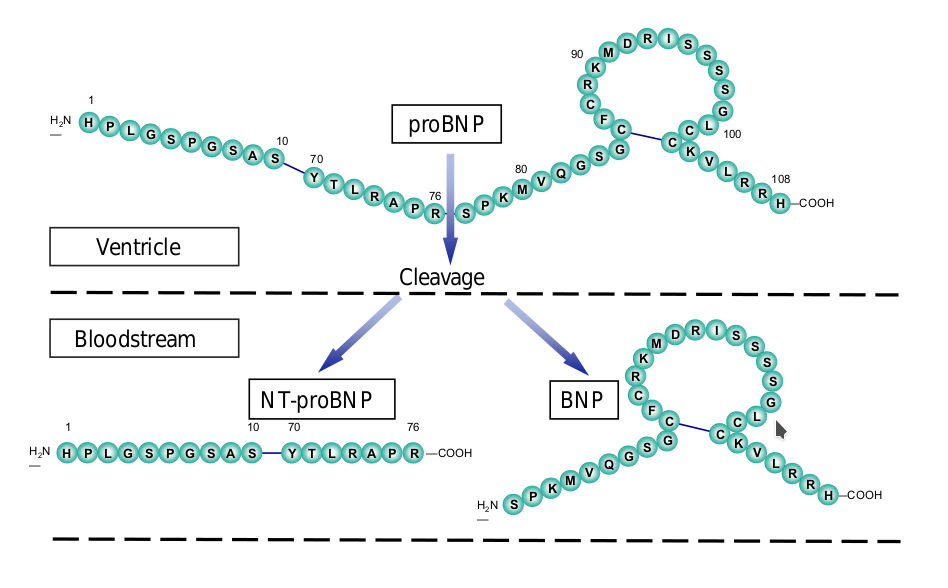
\includegraphics[scale=0.4]{../../images/BNP_secretion.png}

    \small\caption{Secretion of BNP and NT-proBNP}

    \label{BNP_secretion}

\end{figure}



\subsubsection{BNP and NT-proBNP in clinical practice}



Recent trials provided strong evidence that BNP and NT-proBNP are powerful diagnostic tools in exclusion and diagnosis of HF. The Breathing Not Properly study showed, by means of receiver operating characteristics analyses, that a BNP value of 100 pg/ml was the optimal value to differentiate patients with dyspnoea caused by HF from patients with dyspnoea due to pulmonary pathology at the emergency department Fig. \ref{BNP_ER} and \ref{NTBNP_ER}.  This value of 100 pg/ml also discriminated non-systolic HF (LVEF <45\%) from non-HF patients at the emergency department. \citep{Maisel2002}



 An international pooled analysis of 1256 patients provided cut off values for NT-proBNP in an emergency department setting. An age independent cut point of 300 pg/ml had a negative predictive value of 98\%.  Additionally, an optimal strategy to identify acute HF was to use age stratified cut off points of 450, 900 and 1800 pg/ml for ages <50, 50-75, and >75 respectively which yielded 90\% sensitivity and 84\% specificity for acute HF. \citep{Januzzi2006a}

 BNP and NT-proBNP seem useful as diagnostic tools in primary care (where most patients with suspected HF are encountered and where only limited diagnostic tools are available) and as such are recommended in 2005 european guidelines for the diagnosis and treatment of chronic heart failure. \citep{Swedberg2005}





\begin{figure}

    \centering

    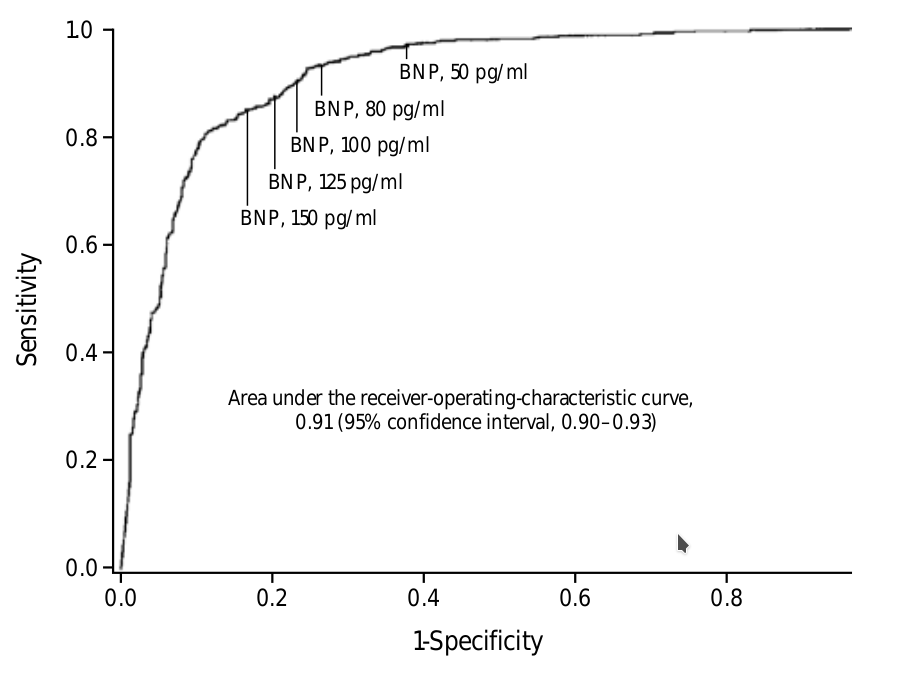
\includegraphics[scale=0.4]{../../images/BNP_ER.png}

    \small\caption{ROC curves for BNP in the diagnosis of heart failure at the emergency department \citep{Januzzi2005}.}

    \label{BNP_ER}

\end{figure}



\begin{figure}
    \centering
    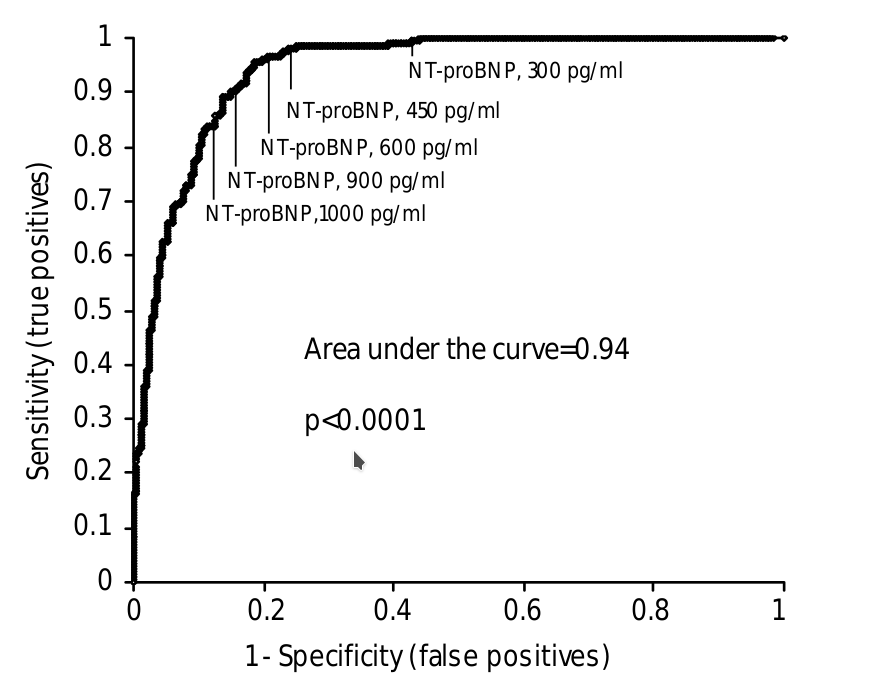
\includegraphics[scale=0.4]{../../images/NTBNP_ER.png}
    \small\caption{ROC curves for NT-proBNP in the diagnosis of heart failure at the emergency department.\citep{Januzzi2005}}
    \label{NTBNP_ER}
\end{figure}





\textbf{Prognosis}



\citep{Tsutamoto1997} in a study on 85 patients with chronic HF revealed that BNP is a strong independent predictor of mortality.  \citep{Berger2002} confirmed these results in a larger research population of 452 systolic HF patients (LVEF <35\%). In this study BNP was found to be a strong independent predictor of sudden death during a follow up period of 3 years.



\citep{Hartmann2004} in a substudy of the COPERNICUS trial (n=1011) revealed that NT-proBNP was consistently associated with an increased risk for all-cause mortality and hospitalisation for HF in patients with severe HF (LVEF <25\%). \citep{Gardner2003b} studying 142 patients with advanced HF also reported that NT-proBNP was an independent predictor of all cause mortality.





\textbf{Guidance of treatment}



BNP and NT-proBNP are influenced by drugs that are prescribed to HF patients like diuretics, beta blockers, ACE inhibitors or angiotensine II receptor blockers and therefore these natriuretic peptides could possibly be used to guide medical treatment. A small study by the Australia-New Zealand Heart Failure Group including 69 patients with symptomatic HF provided evidence of the possible benefit of a NT-proBNP guided approach to therapy. Half of the patients received therapy guided by plasma NT-proBNP, therapy in the remaining patients was guided by clinical monitoring at the same frequency, but with the physician blinded to the NT-proBNP result.

The study found significantly lower mortality, fewer hospitalisations and episodes of decompensated HF in the NT-proBNP-guided therapy group (target 1680 pg/ml). \citep{Troughton2000}



\subsubsection{Variables influencing BNP and NT-proBNP levels: potential limitations?}

Although natriuretic peptide levels are of value in the diagnosis and prognosis of HF patients, several clinical conditions other than HF influence BNP and NT-proBNP plasma levels as well. These influences may be a disadvantage for the use of BNP and NT-proBNP in clinical practice of HF since it may lead to biased interpretations of the test results.



BNP and NT-proBNP are also elevated in patients with acute coronary syndrome. After acute myocardial infarction, levels of BNP rise rapidly during the first 24 hours and then tend to stabilize, \citep{deLemos2001} and in patients with a Q-wave infarction, a peak in NT-proBNP levels was found after 12-48 hours. \citep{Talwar2000}

Moreover, atrial fibrillation resulted in increased BNP levels in patients without, but not in patients with HF. \citep{Knudsen2005} Right ventricular failure due to acute pulmonary embolism can also be determined by BNP. \citep{Tulevski2002} Furthermore, hypertensive patients have higher BNP and NT-proBNP levels compared to non-hypertensive subjects. \citep{Boomsma2001}



A few studies in relatively small study populations without HF showed that anaemia causes elevated BNP levels \citep{Tsuji2004,Willis2005,Wold2005} and in a study on a small group of HF patients anaemia was also related to increased NT-proBNP levels. \citep{Wu2005}

Since both BNP and NT-proBNP are known to be elevated in case of renal dysfunction, \citep{Luchner2005}

In several large studies lower natriuretic peptide levels were associated with higher body mass indexes. \citep{Das2005,Krauser2005,Mehra2004,Wang2004b} As far as diabetes is concerned, results are conflicting between BNP and NT-proBNP; BNP levels did not differ between patients with or without diabetes, \citep{Wu2004} but NT-proBNP levels seem to be higher in diabetic patients compared to non diabetics. \citep{Magnusson2004}

Furthermore, ascitic cirrhosis, hyperaldosteronism, hypercortisolism, carcinoma, subarachnoid hemorrhage, \citep{Pfister2004} are clinical conditions with reported elevated natriuretic peptide levels.



Studies showed that both BNP and NT-proBNP levels are influenced by biological variation, with the biological variation of BNP being higher compared to NT-proBNP (up to 44\% and up to 35\% respectively). \citep{Bruins2004,Wu2003b}

Both BNP and NT-proBNP increase with advancing age and are higher in females compared to males in healthy subjects. \citep{Raymond2003}



\section{Clinical Considerations and Applications in Cardiac Diseases}

\subsection{ Circulating Levels of Cardiac Natriuretic Hormones}

\subsubsection{Physiological Considerations and Clinical Interpretation}

\subsubsection{ Influence of Age and Gender}

The circulating levels of NPs are regulated or modified by several physiological factors

(such as circadian variations, age, gender, exercise, body posture, and water immersion),

eating habits (especially sodium intake), clinical conditions (Table 5.1), and drugs (including corticosteroids, sex steroid hormones, thyroid hormones, diuretics, angiotensin-converting enzyme [ACE] inhibitors, and adrenergic agonists and antagonists) \citep{bib31} \citep{bib32} \citep{bib33} \citep{bib34} \citep{bib35} \citep{bib36}.



The wide variations of circulating levels of NPs in adult healthy subjects in relation to aging and gender could have a particular clinical relevance (Figs. 5.1 and 5.2, Table 5.2).

In order to explain these variations, the possible influence of sex steroid hormones on the NPs system, as well as the modification of the cardiovascular system with aging, should be taken into account. According to these mechanisms, the higher NPs values of women during the fertile adult period could be explained by the physiological stimulation of female sex steroid hormones. In particular, the BNP concentration is on average 36\% higher in women than in men aged less than 50 years \citep{bib37} (Figs. 5.1 and 5.2, Table 5.2).



 The increase in NPs with aging may be due to the decline in myocardial function and other organs (including kidney), typical of senescence. In this case, the NPs assay may be considered as a biochemical marker of increased risk of cardiac morbidity in old age \citep{bib316}.  The increase in NPs with aging may also be due to a decrease in their clearance rate. Indeed, an age modulation of maximum binding capacity of clearance (C-type) receptors for NPs was reported in platelets of elderly persons \citep{bib317}.



All NPs derive from pre-pro-hormones (i.e., preproANP and preproBNP), containing a signal peptide sequence at the amino-terminal end. The pro-hormones (i.e., proANP and proBNP) are produced by cleavage of signal peptide, and then are further split into inactive longer NH-2 -terminal fragments (i.e., NT-proANP or NT proBNP), and a biologically active shorter COOH-terminal peptide (i.e., ANP or BNP), which are secreted in the blood in equimolar amounts (Figs. 3.11 and 3.12). However, ANP and BNP have a shorter plasma half-life and consequently lower plasma concentration, compared to NT-proANP and NT-proBNP (Table 4.1) \citep{bib35} \citep{bib36} \citep{bib37}



Studies on structure-activity relationships have shown the importance for the binding to the specific receptors of the central ring structure of NPs, formed by a disulfide bridge between the two cysteine  residues. For this reason, only ANP and BNP, which present the disulfide bridge in the peptide chain, share the typical hormonal activity of NPs, while the NT-proANP and NT-proBNP do not \citep{bib35} \citep{bib36} \citep{bib37}.



Theoretically, setting up an immunoassay for NT-proANP and NT-proBNP should be easier because their plasma concentrations are higher than ANP and BNP.  On the other hand, NT-proANP and NT-proBNP immunoassays may be affected by several analytical problems, mainly concerning the different assay specificities; consequently, very different results are produced by different methods with a large bias (Table 4.1). The different analytical performance might affect the diagnostic accuracy of the assays, in discriminating between subjects with or without cardiac disease \citep{bib32} \citep{bib35} \citep{bib36}.



The respective advantages of measuring biologically active peptide hormones (ANP and BNP), or inactive peptides (NT-proANP and NT-proBNP) are summarized in Table. The assay of the inactive propeptides better fits the definition of disease marker than the assay of circulating levels of ANP or BNP, which, on the other hand, may be considered a more reliable index of the activation status of the NPs system. Considering the biochemical and physiological characteristics of the different peptides, it is conceivable that ANP is a better marker of acute overload and/or rapid cardiovascular hemodynamic changes than BNP and, especially, than NT-proANP or NT-proBNP \citep{bib32} \citep{bib35}.



\subsubsection{ Resistance to the Biological Action of NPs}



Patients with chronic HF show increased NPs plasma levels compared to normal subjects (Table 3.1, Fig. 3.13). These findings have been defined the “endocrine paradox” in HF, i.e., extremely high circulating levels of hormones with powerful natriuretic activity in patients with congestive HF, who show physical signs of fluid retention and vasoconstriction due to a relatively poor biological activity of the NPs system \citep{bib36}.



A blunted natriuretic response after pharmacological doses of ANP and BNP has been observed in experimental models and in patients with chronic HF, suggesting a resistance to the biological effects of NPs, principally natriuresis \citep{bib325} \citep{bib333} \citep{bib331}. This resistance syndrome was also demonstrated by in vivo turnover studies using radioactive tracers in patients with HF \citep{bib333}.



Resistance to the biological action of NPs could, theoretically, have three different causes (Table 5.3). First, circulating NPs could be, at least in part, inactive. Furthermore, a great fraction of NPs could be inactivated by plasma and tissue proteases before they bind to specific receptors. These two conditions account for all possible mechanisms acting at the pre-receptor level. Second, down-regulation of specific receptors could explain a reduced NPs activity. Finally, some mechanisms can act at postreceptor level, counteracting the biological effects of NPs.



\strong{Mechanisms acting at pre-receptor level}



Some peptides, derived in vivo or in vitro from degradation of intact proBNP, are biologically inactive, although they can be measured by immunoassay methods. Since the circulating levels of intact proBNP and of its derived peptides increase progressively with severity of HF, immunoassay methods can greatly overestimate the true biological activity of NPs in patients with severe HF. Unfortunately, at present, it is not possible to estimate the inaccuracy of NPs immunoassays because these methods use different, not standardized antibodies and calibrators, leading to highly different clinical results \citep{bib36}.



A resistance to the biological action of NPs may be theoretically due to an increase in degradation (turnover) of circulating biologically active peptides. NPs are degraded in vivo and in vitro by several types of proteolytic enzymes, including serin-proteases, peptidyl arginine aldehyde proteases, kallikrein like proteases, and neutral endopeptidases (NEP) \citep{bib335}.



Individual differences in the ability of heart tissue to mature the precursor of NPs peptides, or of peripheral tissues to degrade them, may help to explain why there are some differences in the clinical presentation among patients with HF with similar clinical severity and ventricular function \citep{bib36}.



From a clinical point of view,it is important to note that some drugs sharing an inhibitory action on both NEP and ACE (so called vasopeptidase inhibitors) may have some beneficial effects in patients with arterial hypertension and/or HF because the administration of these durgs can potentiate the biological activity of NPs system by increasing the concentration of biologically active peptides \citep{bib340} \citep{bib341} \citep{bib342}.



It is important to note that renal function can affect the biological action of NPs in different ways .CNH are small peptides freely filtrated by renal glomerulus; the kidneys are probably responsible for about 50\% of metabolic clerance rate of plasma ANP and BNP and in this way renal diseases can affect the circulating levels of NPs.  Indeed,a decreased renal function greatly increases the plasma NPs concentration and consequently more peptide hormones are available for other target tissues (such as brain,vascular tissue,adrenal gland and so on) \citep{bib35}.



Luminal perfusion with ANP has been shown to reduce sodium efflux from the inner medullar collecting duct, suggesting that this hormone has also luminal sites of action.  As a consequence, a reduction in the filtration can potentially induce renal hypo-responsiveness to NPs \citep{bib325}.



Some studies suggest that the resistance to biological effects of NPs in HF may be due,in part,to variations in the relative amount of the three different types of natriuretic peptide-specific receptors.In particular,there could be an upregulation of type C receptors (NPR-C) with a parallel down regulation of type A and B receptors (NPR-A and NPR-B) \citep{bib343} \citep{bib347}.



NPR-A and NPR-B mediate all known hormonal actions of NPs, therefore their down-regulation should induce a deactivation of the NPs system. The upregulation of NPR-C receptors that strongly contribute to the clearance of biologically active peptides could further increase the resistance to NPs in patients with HF \citep{bib343}.



These findings are well in accordance with the results of in vivo kinetic studies obtained using radioactive tracers in patients with HF \citep{bib333}. Reversal of cardiomyocyte hypertrophy during left ventricular assist device support was accompanied by normalization of ANP, BNP and NPR-C mRNA levels and a significant recovery of responsiveness to ANP \citep{bib347}.



However,  \citep{bib348} found that neither NPR-A nor NPR-B were internalized or degraded in response to natriuretic peptide binding in cultured cells. % move to NPR physiology



Another well-characterized deactivation mechanism is the process by which an activated receptor is turned off, commonly referred to as “desensitization”. Phosphorylation of the intracellular kinase homology domain of NRP-A and NPR-B is required for hormone-dependent activation of the receptor, while dephosphorylation at this site causes desensitization. Deactivation of the NPs system via desensitization of NRP-A and NPR-B can occur in response to various pathophysiological stimuli \citep{bib348}.% \citep{bib349}



% Further studies are necessary to clarify what is the most important mechanism of deactivation of NPs system acting in vivo at receptor level in patients with heart failure: the down-regulation (of NPR-A and NPR-B), the upregulation (of NPR-C), or the desensitization (of NPR-A and NPR-B).



A peripheral resistance to the biological effects of NPs may play an important role in other clinical conditions, besides HF. For example, NPR-C is also present on cellular membranes of adipose tissue. It was suggested that the increase in NPR-C receptors observed in obese subjects can in turn increase the peripheral degradation of NPs and consequently blunt the action of the NPs system. This reduced activity of the NPs system may increase the risk of developing arterial hypertension and other cardiovascular diseases due to the non-contrasted and therefore prevailing effects of the counter regulatory system with sodium-retentive and vasoconstrictive properties \citep{bib352}.



However, the NPR-C receptor could be coupled to a G-protein that inhibits cyclic AMP synthesis. These receptors, which are present in great amount especially on the endothelial cell wall, may mediate some paracrine effects of CNP on vascular tissue \citep{bib355}.



Studies demonstrated that the activation of the neuro-hormonal system accelerates the left ventricular functional impairment in patients with HF. Drugs that contrast the detrimental effects of the neuro-hormonal system activation play a key role for the current pharmacological treatment of HF. Some of these, such as ACE inhibitors, angiotensin II receptor blockers, $\beta$-blockers, and spironolactone decrease the circulating levels of NPs,“normalize” their kinetics, and increase their biological activity \citep{bib35}. Furthermore, they enhance the natriuretic effect of ANP or BNP analogs administered to patients. In other words, the treatment with this type of pharmacological agents decreases the systemic resistance to the biological effects of NPs \citep{bib333}.



Patients with HF show a progressive and parallel increase in NPs levels and in some neuro-hormones and cytokines. This increase can be closely related to disease severity, as assessed by functional NYHA class (Table 3.1, Fig. 3.13). Plasma BNP values, normalized by mean values found in healthy subjects, are significantly higher than other normalized neuro-hormone and cytokine values in HF (Fig. 5.3, Table 5.4) \citep{bib360}.



On average, the response of the NPs system to the increasing challenge of disease severity may not be linear (Fig. 5.4). The curve reported in Figure 5.4 suggests that the NPs system responds with a sharp increase in BNP plasma concentration in the early phase of HF (NYHA class I-II patients), followed, with the clinical progression of the disease, by a blunted increase (NYHA class III), and finally by a plateau (NYHA class IV) (Table 3.1, Fig. 5.4) \citep{bib333}.



\subsubsection{ Diagnostic Accuracy of NPs Assay in Plasma from Patients with Cardiac Diseases}



The NPs system activation is modulated not only by hemodynamic factors, but also by the activity of the counter-regulatory neuro-hormonal system. Consequently, it is likely that very small changes in hemodynamics, not assessable by echocardiographic examination, may produce significant (and measurable) variations in plasma concentrations of NPs \citep{bib360}. (Fig. 5.3).



It is well known that changes in hemodynamic parameters (such as left ventricular ejection fraction, EF) and plasma NPs levels (expressed in a log scale) are closely related in patients with cardiovascular diseases (Fig. 5.5) \citep{bib32} \citep{bib33} \citep{bib34} \citep{bib35}  \citep{bib360} \citep{bib363} \citep{bib364}.



However, correlations between plasma NPs levels and echocardiographically measured parameters, such as left ventricular EF, myocardial mass and chamber volumes, are usually less close in the general population (large community-based sample, including healthy subjects with or without individuals with asymptomatic myocardial dysfunction) \citep{bib38} \citep{bib39} \citep{bib366} \citep{bib367}. Figure 5.6.



It should be emphasized that the recognition of HF syndrome is not equivalent to the clinical diagnosis of cardiomyopathy or to the assessment of left ventricular dysfunction, these latter terms describing possible structural reasons for the development of HF. Instead, HF is a clinical syndrome that is characterized by specific symptoms (dyspnea and fatigue) and signs (fluid retention). There is no diagnostic test for HF, because it is largely a clinical diagnosis based on a careful history and physical examination. Therefore, there are no objective criteria for the identification and/or clinical stratification of patients with suspected HF; several “reference standards”, based on clinical, laboratory and instrumental examinations, can be used to evaluate the diagnostic accuracy of the NPs assay. Thus, some studies took into consideration only echocardiographic assessment of ventricular dysfunction, while in others either results of echocardiography or all clinical data have been used for the diagnosis of HF.  Unfortunately, using echocardiography as the unique reference standard may lead to misinterpretations when evaluating the diagnostic accuracy of the NPs assay. A systematic review of clinical studies in patient populations with a prevalence of HF ranging from 3.8\% to 51\% to determine the diagnostic accuracy of BNP assays found that the sensitivity (ranging from 90 to 97\%) was much less variable (by 4.4-fold) than the specificity (ranging from 53 to 84\%) \citep{bib35}.



Furthermore, in a meta-analysis by \citep{bib372}, diagnostic accuracy of BNP assays greatly varied according not only to the group of patients studied, but also to the reference standard used (left ventricular EF <40\% or <55\%, diagnosis of diastolic dysfunction, diagnosis of systolic + diastolic dysfunction, or integrative clinical criteria). These data indicate that the choice of a suitable and accurate reference standard for evaluation of the diagnostic accuracy of the BNP assay in patients with HF may be a problem that is actually underestimated in the literature. For a proper definition of diagnostic accuracy, tested individuals should be grouped into those with and without disease, by means of an independent clinical judgment.



Careful echocardiographic examinations usually show slightly better or even similar diagnostic accuracy than the BNP assay in patients with cardiac diseases \citep{bib3178}.



On the other hand, the NPs assay may have some advantages compared to echocardiographic examinations alone in specific clinical settings. For example, \citep{bib375} suggested that in patients with chronic HF, the NT-proBNP assay reflects functional cardiac impairment and decreased exercise capacity (measured by peak exercise oxygen consumption) better than the left ventricular EF.



Several studies indicate that BNP and NT-proBNP are powerful and independent risk markers of cardiovascular events (especially mortality) not only in patients with HF, but also in those with acute coronary syndrome, as reported in  and systematic reviews \citep{bib35} \citep{bib376} \citep{bib377} \citep{bib378}. Some studies also suggested that the cardiovascular risk increases progressively to NPs concentration \citep{bib377} \citep{bib378} \citep{bib3194}; that is, there is no threshold that actually identifies patients with null risk.



Diagnostic sensitivity of BNP/NT-proBNP assays in detecting left ventricular systolic dysfunction could be suboptimal in asymptomatic or low-risk individuals, especially in women \citep{bib39}.



Specificity of BNPassays in patients with HF ranged from 53 to84\% and positive predictive values from 3 to 85\% inseveral studies. These data indicate that NPs assays can produce a relatively large number of false-positive results. Consequently, many individuals, actually without HF (about 15-60\% of those with positive NPs tests),mightundergo expensive and/or harmful investigations to rule out the disease, or even be inappropriately labeled as cardiac patients \citep{bib35}.



Several false-positive results can be observed in patients with various clinical diagnoses, as reported in Table 5.1. In these patients, increased plasma BNP may predict, even in the presence of a normal echocardiographic examination, an increased risk of mortality or major cardiac events, including pulmonary embolism \citep{121} \citep{123} \citep{bib382} and hypertension \citep{bib383}, renal failure \citep{bib384} \citep{bib385}, septic shock \citep{bib386}.



On the other hand, false-negative results could be found in patients on treatment with anti-adrenergic agents, diuretics and/or ACE inhibitors, all drugs that can reduce NPs levels \citep{bib35}. As shown in Figure 5.7, a large number of patients with only mild HF (NYHA classes I and II) may have values slightly above or even under the 99th percentile of distribution values of BNP concentration in healthy subjects. In these patients, successful treatment and consequent improvement in cardiac function and exercise capacity, and reduction in filling pressure and cardiac volumes, is usually associated with a marked fall in NPs levels: thus, a larger number of patients could have BNP values within the reference range values \citep{bib35} \citep{bib390}. %check if bib390 is the reference for the figure



However, at matched echocardiographic alterations, patients in whom BNP levels drop in response to therapy have a reduced rate of major cardiac events or mortality, compared to untreated hypertensive patients, who could have similar echocardiographic abnormalities. This represents the rationale for using the NPs assay for therapy decision making and for monitoring HF patients \citep{bib35} \citep{bib363} \citep{bib364}.



In populations with a higher prevalence of cardiac diseases, including only individuals with a clinical suspicion of HF, the diagnostic sensitivity of BNP can improve up to 95\%, or even more, as long as appropriate cut-off values are selected \citep{bib35} \citep{bib372}. In this case, a strategy called “SnNout”, which maximizes test sensitivity, could be used to rule out the presence of HF \citep{bib391}.



Furthermore, NPs assay also shows high (>95\%) negative predictive values \citep{bib35} \citep{bib320}, which can help to confirm the absence of HF. This is the rationale for choosing the NPs assay as the first step for an algorithm for the diagnosis of HF \citep{bib369} \citep{bib370}. Such a clinical strategy has proved successful in some  studies evaluating the cost-effectiveness of using plasma BNP measurements for screening of cardiac dysfunction in the general population \citep{bib392} \citep{bib393} \citep{bib3171}.





\subsubsection{ Biological Variation of Plasma BNP: a Problem or a Clinical Resource?}



The variability of measured plasma concentrations of many substances is due to three different sources: pre-analytical, analytical and inherent biological variation. The latter is usually described as a random variation around a homeostatic setting point, and defined as the intra-individual or within-subject biological variation \citep{bib395}.



% Several physiological parameters and endogenous substances are closely regulated by complex biological mechanisms in such a way as to vary little. If a random variation is assumed for an analyte, the effect of imprecision on dispersion can be taken into consideration for setting generally applicable quality specifications for assay performance in order to indicate an acceptable (or desirable) degree of assay precision. Accordingly, the desirable assay imprecision should be equal to or less than half of the intra-individual biological variation \citep{bib397}.



In order to achieve a correct interpretation of serial test results that are collected for follow-up or tailored treatment of HF patients, several studies evaluated the biological variation of BNP and its related peptides, in both healthy subjects and cardiac patients. Due to secretory bursts and its rapid turnover (half-life about 15-20 min), intra-individual biological variations of plasma BNP levels were found to be very large, in both healthy subjects and patients with heart failure (ranging from 30 to 50\%) \citep{bib399}.  %Assuming a random variation around a homeostatic setting point, the calculated reference change values at 95\% confidence interval ranged from 99 to 130\% for BNP in healthy subjects and patients \citep{bib397} \citep{bib399} \citep{bib3100} \citep{bib3101}.

According to this, only a decrease of more than 50\% or a more than 2-fold increase in plasma BNP should be assumed to be statistically significant in an individual patient.



In contrast with this assumption, a clinical trial \citep{bib390} has suggested that a BNP decrease inferior to this calculated reference change could be clinically relevant in patients with heart failure. In this study, only the group of patients treated with the \beta-blocker agent carvedilol, who respond on average with a decrease of only 38\% in plasma BNP, showed a clinical improvement \citep{bib390}.



Furthermore, several studies have demonstrated that cardiovascular risk (mortality or major cardiovascular events) increases continuously and progressively throughout the whole range of BNP concentrations in patients with cardiovascular diseases \citep{bib35} \citep{bib377} \citep{bib378} \citep{bib3194}.



In order to explain these conflicting findings, it should be taken into account that BNP secretion is closely regulated by specific pathophysiological mechanisms.  According to this hypothesis, the clinician should consider all changes in BNP concentration as potentially clinically relevant, even when narrower than the calculated intra-individual biological variation \citep{bib3103}.

In other words, BNP variations should be interpreted and considered by physicians, as the variability of heart rhythm and blood pressure, by taking into account clinical history and examination, comprehensive of the response to specific treatments, as well as of laboratory and instrumental test findings.



\subsection{ NPs Assay as Diagnostic and Prognostic Tool in Cardiac Diseases}



\subsubsection{ Use of NPs Assay in the Screening and Classification of Patients with Cardiac Dysfunction}



The diagnosis of HF can often be difficult, mainly in primary care settings, where patients may present with non-specific symptoms and signs, such as dyspnea, fatigue, and ankle swelling. In several population-based studies, fewer than 40\% of patients with a suspected diagnosis of HF in primary care had this diagnosis confirmed by more specific and accurate clinical investigations, which are often expensive, timeconsuming and demanding for the patient \citep{bib369} \citep{bib370} \citep{bib3105}. As a result, a relatively simple and inexpensive biochemical test (such as the NPs assay) may be very useful to confirm the clinical suspicion of HF in this clinical setting \citep{bib35} \citep{bib3131} \citep{bib335}.



\subsubsection{ Diagnostic Accuracy of NPs Assay in Asymptomatic,}

\strong{Screening in general population}

\citep{bib39} analyzed the Framingham Heart Study cohort (3,177 individuals) using BNP and NT-proANP in the evaluation of left ventricular hypertrophy and systolic dysfunction in a community population.  The presence of the disease was evaluated by using echocardiographic findings (the prevalence of left ventricular systolic dysfunction was 9.3\% in the 1,470 men and 2.5\% in the 1,707 women tested, respectively). The area under the curve (AUC) of receiver operating characteristic (ROC) analysis for NPs assay for identifying both left ventricular hypertrophy and systolic dysfunction was on average about 0.75, with a good specificity (assumed 95\% both for men and women) and negative predictive value (NPV, on average ranging from 92\% to 97\% in men, and from 91\% to 98\% in women), but a poor sensitivity (i.e., ranging from 27\% to 28\% in men, and from 13\% to 40\% in women) and positive predictive value (PPV, from 22\% to 38\% in men, and from 5\% to 40\% in women), using gender-related BNP cut-off values \citep{bib39}.

The aim of \citep{bib366} was to examine the validity of plasma BNP measurement for detection of various cardiac abnormalities in a rural Japanese population (1,098 subjects, 693 men and 405 women), with a low prevalence of coronary heart disease and left ventricular systolic dysfunction (i.e., only 37 participants, corresponding to 3.0\%, showed an EF <30\%). The diagnosis was carried out by two independent cardiologists based on a medical questionnaire, chest radiogram, electrocardiogram (ECG), and echocardiographic report. The optimal threshold for identification of disease was a BNP concentration of 50 ng/l (14.4 pmol/l), with an area under the ROC curve of 0.970, a sensitivity of 89.7\%, a specificity of 95.7\%, PPV of 44.3\%, and NPV of 99.6\%, respectively.

The conclusions of these two studies, though similar in aim, as well as in clinical and experimental protocols, were strongly conflicting. The Japanese study suggested that the BNP assay is a very efficient and cost-effective mass screening technique for identifying patients with various cardiac abnormalities regardless of etiology and degree of left ventricular systolic dysfunction, while the Framingham study suggested only limited usefulness of the NPs assay as a mass screening tool for this clinical condition, especially in women.  This discrepancy may be due to the different standard used for the diagnosis of heart failure adopted in the two studies, as discussed in a previous paragraph . However, these two studies, taken as a whole, indicate that the NPs assay may have only a limited usefulness as a screening method for HF in a general population, owing to the poor sensitivity and PPV. However, both studies also found good specificity and NPV, thus suggesting that the NPs assay may be used to rule out HF in an asymptomatic individual.

\subsubsection{ Diagnostic Accuracy of NPs Assay in Patients with Suspected HF}

Many studies have suggested that the NPs assay could be useful as a screening method and/or for the differential diagnosis in patients suspected of HF in different clinical settings:

\begin{itemize}

  \item randomly selected high-risk community populations

  \item primary-care patients with a new diagnosis of HF

  \item patients with acute dyspnea in the emergency department

  \item consecutive unselected hospital inpatients

  \item patients admitted to the intensive care unit.

\end{itemize}



The studies concerning the diagnostic accuracy of the NPs assay in patients with HF have also been analyzed by two systematic reviews \citep{bib35} \citep{bib372}; unfortunately, these studies showed quite heterogeneous data, thus introducing some bias in the statistical analysis. Even some high quality studies were not designed with the primary goal of evaluating the diagnostic accuracy of the NPs assay, where this aim was considered only at a post-hoc analysis and retrospectively assessed in blood samples collected for different original purposes, some years before the actual evaluation of diagnostic accuracy. This may introduce a significant bias, although its true clinical relevance is difficult to assess \citep{bib35}.



The second most important cause of heterogeneous data is the different reference standard used to evaluate the diagnostic accuracy of the NPs assay. In some studies, the patients studied were stratified and grouped according to clinical severity, as described by functional classification (usually NYHA classification). In other studies, only echocardiographic measurements were used as “standard” for the accuracy of the NPs assay for the diagnosis of left ventricular dysfunction (and not for the clinical diagnosis of HF) \citep{bib372}.



Furthermore, comparison of studies concerning the diagnostic accuracy of NPs assay is also difficult because different populations were enrolled and different immunoassays were used. Indeed, diagnostic accuracy (especially predictive values) is strictly dependent on disease prevalence (pre-test probability), which greatly varies according to the clinical setting considered (i.e., screening for general population, out-patients seen by a general practitioner, or in primary care, emergency department, coronary care unit, and so on). In particular, the prevalence of HF in the populations studied varied from less than 5\% (in studies of screening of asymptomatic population) to more than 50\% (in studies including patients referred to hospital with suspicion of HF) \citep{bib35}.

%Unfortunately, some studies do not clearly indicate the type of immunoassay used to measure NPs, while the majority do not report the assay performance (and often even the reference values) evaluated in their own laboratory.\citep{bib35}

Taking all studies as a whole, a meta-analysis showed that the odds ratio for diagnostic accuracy of BNP assay in different groups of patients with suspected HF is highly significant. In particular, the pooled diagnostic odds ratio, when clinical criteria were used as gold standard for HF, was 30.9 (95\% confidence interval 27.0-35.4), while it fell to 11.9 (8.4-16.1) when a value $\leq$40\% of left ventricular EF, was used as reference standard \citep{bib372}.

Including data of three studies comparing the diagnostic accuracy of BNP assay in patients with diastolic dysfunction, the pooled odds ratio was 28.3 (95\% confidence interval 2.66-300.5). However, a bias may affect these studies, as suggested by the significant test of heterogeneity \citep{bib372}.

\citep{bib3133} evaluated the effect of NT-proBNP assay on the clinical diagnostic accuracy of HF in primary care by means of a prospective, randomized controlled trial in 305 patients. Each patient was randomized in two groups, one in which the general practioner had at their disposal the NT-proBNP assay results (NT-proBNP assay group), while the other did not (control group). The diagnostic accuracy improved by 21\% in the NT-proBNP assay group and by 8\% in the control group (p = 0.002). This study indicates that NT-proBNP measurement significantly improves the clinical diagnostic accuracy of HF in general practice.

\subsubsection{Diagnostic Accuracy of NPs Assay in Patients with Acute Myocardial Infarction}

Circulating levels of NPs increase after acute myocardial infarction (AMI); the extent of the increase is related to the size of the infarct. Patients with smaller infarcts tend to have a monophasic increase in plasma BNP, peaking at 20 hours after the onset of symptoms; on the other hand, those with larger infarcts, lower EF, and clinical signs of HF may present a further peak at 5 days after admission. Other studies are less convincing regarding the ability of the NPs assay to identify patients with significant myocardial dysfunction after AMI \citep{bib3139}. These conflicting results could be due to the differences in sample collection time, type of NPs (ANP, BNP, or NT-proBNP) measured, type of assay, and inclusion criteria adopted. However, persisting elevation of NPs levels at 1 or 2 months after AMI usually suggests a high risk of adverse remodeling and subsequent HF \citep{bib35}.

The diagnostic accuracy of the BNP assay in patients with myocardial infarction was evaluated in the meta-analysis by \citep{bib372} taking into account only two studies \citep{bib3140} \citep{bib3177}, fitting the inclusion criteria of this analysis; the pooled odds ratio was 9.4 (95\% confidence interval 4.5-19.4).



\subsubsection{ Diagnostic Accuracy of NPs Assay in Elderly People}



Heart failure is primarily a disease of old age; chronic HF increases in prevalence with aging from <1\% in people aged <65 years to >5\% in those >65 years of age, and this clinical condition is the first cause of morbidity and mortality in older people. \citep{bib3193} demonstrated that elderly patients present with more advanced HF, as evidenced by their higher morbidity and mortality rate along with greater neurohormonal activation . According to these findings, elderly people should be considered to be a population with high risk for developing HF and so the BNP/NT-proBNP assay may be useful as a screening test for HF in older age.

\citep{bib3143} in a prospective study specifically evaluated the diagnostic accuracy for HF of BNP assay in 299 consecutive patients (mean age 79 years, 65\% women) attending day-hospital over a period of 13 months. This study suggested that both BNP assay and ECG were sensitive in detecting left ventricular systolic dysfunction, but lacked specificity (but the combination of the two tests improved diagnostic accuracy).



\citep{bib3172} reported that both the ECG and the plasma concentration of BNP were highly efficient in excluding left ventricular systolic dysfunction in 407 75-year-old subjects. However, compared with the BNP, the ECG yields a lower number of false-positive cases. Therefore, this study suggested that in screening for left ventricular systolic dysfunction in elderly people, the BNP assay has a diagnostic value in addition to the ECG, but only in individuals with abnormal ECG.

\citep{bib3146} indicated that the BNP assay may be particularly useful in elderly patients, especially in differentiating cardiogenic pulmonary edema from respiratory causes of dyspnea.

Screening of populations with more than 1\% prevalence of HF (such as people with age more than 60 years) with BNP followed by echocardiography should provide a health benefit at a cost that is comparable to or less than other accepted health interventions \citep{bib3145}.

\citep{bib3147} demonstrated that NT-proBNP assay was useful for detecting HF among people living in elderly nursing homes.


Another example of the clinical relevance of BNP assay is the possibility of identifying HF caused by drug cardiotoxicity. Cardiotoxicity is a potential side-effect of some chemotherapeutic agents. The anthracycline class of cytotoxic antibiotics are the most famous, but other chemotherapeutic agents can also cause serious cardiotoxicity and are not so well recognized (including cyclophosphamide and fluorouracil) \citep{bib3154}.

In a large retrospective study of more than 4,000 patients, an incidence of clinical chronic HF of 2.2\% was found \citep{bib3155}. However, another  study suggests that about 20\% of patients treated with anthracycline show a decrease in ventricular function below the normal limits, if followed with serial measurements of left ventricular EF, assessed by an accurate radionuclide method \citep{bib3156}. This supports the recommendations of monitoring cardiac function in anthracycline-treated patients with accurate and suitable methods. Experimental studies in rats indicated that plasma BNP and serum cardiac troponin T (cTnT) significantly increased from 6 to 12 weeks after adriamycin administration with deterioration of cardiac function, as assessed by echocardiography \citep{bib3157}. However, in this study the increase in cTnT was antecedent to the increase in BNP and the deterioration of cardiac function \citep{bib3157}.

\citep{bib3161} and \citep{bib3162} suggested that BNP/NT-proBNP assay is a predictive marker of cardiac dysfunction in patients affected by aggressive malignancies and treated with high-dose chemotherapy. The acute release of circulating levels of troponin should be only a mirror of the death of myocardiocytes, while the persistent increase in BNP, after several days or weeks from the administration of cardiotoxic drug, should be specifically related to ventricular remodeling and myocardial dysfunction.

 \citep{bib3163} \citep{bib3164} suggested that the BNP assay could be a reliable marker of ischemia in patients with coronary artery disease. It could be hypothesized that exercise-induced ischemia results in increased wall stress and triggers release of NPs from myocardiocytes. According to this hypothesis, \citep{bib3163} measured NT proBNP and BNP in blood samples from a group of normal volunteers, and two groups of patients, one with and the other without coronary artery disease, before and after maximal exercise. Post-exercise increases in NT-proBNP and BNP were approximately 4-fold higher in the ischemic group than in the nonischemic group; while in volunteers, the increase was almost identical to that of the non-ischemic patient group. At equal specificity to the ECG (58.8\%), the sensitivities of the BNP/NT-proBNP assay in detecting ischemia were 90 and 80\%, respectively; in contrast, the sensitivity of the exercise ECG was only 37.5\%.

In the study by \citep{bib3164}, transient myocardial ischemia was associated with an immediate rise in circulating BNP levels, and the magnitude of the rise was proportional to the severity of ischemia. These findings demonstrate an important link between the severity of an acute ischemic insult and the circulating levels of BNP. However, further studies are necessary to evaluate the relevance of the BNP/NT-proBNP assay.

\subsection{ Comparison between the Diagnostic Accuracy of NPs Assay and that of Other Tests and Clinical Investigations}

Signs and symptoms correlate poorly with the presence of HF, for this reason diagnosis relies on clinical judgment based on a combination of history, physical examination and appropriate investigation \citep{bib365} \citep{bib369} \citep{bib370} \citep{bib3168}.


\citep{bib392} found that BNP assay showed a diagnostic accuracy better than ECG in a random sample of 1,257 community subjects.  \citep{bib3171} suggested that BNP assay together with the presence of major ECG abnormalities and history reduced by a factor of six (in comparison to consideration of BNP assay in isolation) the number of subjects requiring echocardiography to detect one case of myocardial dysfunction ina large population screening (1,360 patients tested).

In their study, \citep{bib3174} could identify several types of structural heart disease, in particular valvular heart disease, exclusively by BNP testing, suggesting that BNP measurement can make a significant contribution to screening for CHF precursors when used in combination with ECG in elderly populations (856 subjects enrolled, with age $\geq$ 65 years).

However, compared with the BNP assay, the ECG yielded a lower number of false positive cases. In screening for left ventricular systolic dysfunction, the BNP has a diagnostic value in addition to the ECG, but only in individuals with abnormal ECG \citep{bib3172}.

\citep{bib3170} compared the diagnostic accuracy of BNP assay, ECG, chest radiography and echocardiography; the results of this study confirmed that sensitivity, specificity and accuracy of BNP assay and echocardiography were significantly better than those of ECG and chest radiography.

According to the guidelines for the diagnosis of heart failure proposed by the Task Force on Heart Failure of the European Society of Cardiology \citep{bib369}, echocardiography is recommended as the most practical tool to demonstrate cardiac dysfunction. However, in more than 50\% of the clinical studies, the echocardiographic investigation has been considered as the gold standard (more exactly the reference standard method) for the evaluation of diagnostic accuracy of NPs assay in patients with heart failure.  When we use the echocardiography investigation as reference method, we assume that BNP assay cannot theoretically have a better diagnostic accuracy than it. Indeed, conflicting results were found when different clinical settings (patient’s selection) and/or gold standard were used \citep{bib35} \citep{bib372}.

\citep{bib3178} found that BNP assay and comprehensive Doppler echocardiography have similar diagnostic accuracy for congestive HF, although echo-Doppler trended toward higher specificity than BNP for congestive HF.

Serial BNP measurements during the treatment of acute HF provide incremental prognostic information over clinical presentation and repetitive echocardiographic examination \citep{bib3179}.

\citep{bib3180} suggested that both BNP assay and a complete echocardiographic examination do not have adequate discriminatory power to be used in isolation in the evaluation of left ventricular diastolic function. Therefore, all available information, including systolic function, chamber dimensions and all Doppler variables must be considered in the analysis of individual patients.This was in accordance with \citep{bib3181} who assessed the diagnostic performance of BNP testing and echocardiographic assessment of left ventricular systolic function, separately and combined, for the identification of congestive HF in 1,586 patients presenting to the emergency department with acute dyspnea. The proportions of patients who were correctly classified were 67\% for BNP alone, 55\% for EF alone, 82\% for the two variables together, and 97.3\% when clinical, ECG, and chest radiograph data were added. This study suggested that BNP measurement was superior to twodimensional echocardiographic determination of left ventricular EF in identifying congestive HF, regardless of the threshold value. The two methods combined have marked additive diagnostic value.



However BNP/NT-proBNP levels do not accurately predict serial hemodynamic changes and consequently do not obviate the need for pulmonary artery catheterization in patients requiring invasive hemodynamic monitoring \citep{bib3183}.

In conclusion, BNP assay shows significantly higher predictive characteristics than ECG and chest radiography, and a cost-benefit value significantly greater than that of echocardiography \citep{bib392} \citep{bib3170}. BNP measurement may exclude normal heart with high probability owing to its high degree of sensitivity and NPV when used in screening high-risk populations, therefore reducing the echocardiographic diagnostic burden; this is the rationale for considering the BNP assay in the first step of an algorithm for the differential diagnosis of heart failure \citep{bib337} \citep{bib365} \citep{bib369} \citep{bib370} \citep{bib3168} \citep{bib3175}.





\subsection{ Use of NPs Assay as Prognostic Marker in Cardiovascular Diseases}



Several well-designed and conducted studies suggested that the NPs assay may be useful as a prognostic marker mainly in two clinical conditions: HF and acute coronary artery syndromes (ACS), as also demonstrated by systematic reviews \citep{bib35} \citep{bib376} \citep{bib3184} \citep{bib3185}.



\subsubsection{ Prognosis in HF}



The prognostic role of NPs assay (especially NT-proANP, BNP and NT-proBNP) in patients with HF is well demonstrated by a huge number of studies \citep{bib316} \citep{bib3147} \citep{bib3186} \citep{bib3187} \citep{bib3188} \citep{bib3189} \citep{bib3190} \citep{bib3191} \citep{bib3192} \citep{bib3193} \citep{bib3194} \citep{bib3195} \citep{bib3206} \citep{bib3197} \citep{bib3198} \citep{bib3199}.



In all these studies, NPs concentrations were always found to be independent risk markers for morbidity (increased future major cardiovascular events and/or hospitalization) and/or mortality in patients with acute or chronic HF \citep{bib35}. In some studies NPs levels were stronger predictors of mortality and/or major cardiovascular events than left ventricular EF, NYHA class, and/or presence of diabetes or hypertension, as well as sex and age in patients with chronic HF \citep{bib3188} \citep{bib3189} \citep{bib3192} \citep{bib3194} \citep{bib3195} \citep{bib3206} \citep{bib3198} \citep{bib3199}.

% In some  studies \citep{bib3197} \citep{bib3199}, NT-proANP was shown to be a more powerful predictor than BNP and NT-proBNP, but these differences may be due to the analytical performance of methods used rather than a true specific characteristic of peptide measured in the study. Further studies are necessary to clarify whether there is a true difference among the NT-proANP, BNP and NT-proBNP as predictor markers in patients with HF.

A continuous relationship was generally found between BNP levels and mortality \citep{bib3194}, thus suggesting that it is not possible to observe a threshold for the risk. On average, a systematic analysis of the most important studies suggested an odds ratio of about 2 for the risk of mortality in patients with BNP values above the cut-off \citep{bib35}.



% Further evaluation needs the clinical relevance of combined use of NPs assay with other functional parameters (such as peak oxygen consumption) \citep{bib390} \citep{bib3201} \citep{bib3202}, neurohormones \citep{bib3203} \citep{bib3204} \citep{bib3205} \citep{bib3206}, and markers of fibrinolysis \citep{bib3207} or cardiac necrosis \citep{bib3208} \citep{bib3209}.



% Some studies suggest that the combination of BNP assay with the assessment of peak oxygen consumption \citep{bib3202} or with specific markers of cardiac necrosis \citep{bib3209} improves risk stratification of patients with HF. Several studies reported that some neuro-effectors, hormones (including peptide, thyroid and steroid hormones), and cytokines are increased in patients with HF, as  reviewed \citep{bib32} \citep{bib35} \citep{bib3210} \citep{bib3211} \citep{bib3212} \citep{bib3213} \citep{bib3214} \citep{bib3215} \citep{bib3216} \citep{bib3217} \citep{bib3218} \citep{bib3219} \citep{bib3220} .

In general, BNP assay was found to be the most powerful indicator for poor outcome compared to other neuro effectors and hormones, at least in the largest studies \citep{bib35} \citep{bib3204} \citep{bib3206}. However, more data on the clinical relevance of combination of two or more neuro-hormones in risk stratification of HF are necessary.



\subsubsection{ Prognosis in ACS}



Acute coronary artery syndrome encompasses a continuum of cardiac ischemic events, ranging from unstable angina pectoris, with no biochemical evidence of myocardial necrosis, to ST-elevation AMI \citep{bib3221} \citep{bib3222}. The prognosis of patients with ACS varies widely, and several clinical, electrocardiographic, and biochemical markers have been used to identify high-risk individuals in need of aggressive intervention \citep{bib3222}.



Several studies reported that NPs assay (in particular BNP and NT-proBNP) provides valuable prognostic information in patients with ACS \citep{bib3117} \citep{bib3138} \citep{bib3223} \citep{bib3224} \citep{bib3225} \citep{bib3226} \citep{bib3227} \citep{bib3228} \citep{bib3229} \citep{bib3230} \citep{bib3231}. A meta-analysis confirmed the powerful prognostic value of BNP/NT-proBNP in patients with ACS for death both in the short term (<50 days, mean odds ratio 3.38, CI 95\% 2.44-4.68) and long term (>10 months, mean odds ratio 4.31, 3.77-4.94) \citep{bib376}.



% As for the prognostic role of BNP assay in patients with HF, more data on the clinical relevance of combination with other markers in risk stratification of HF are necessary.

Some studies suggest that BNP levels improve a simple risk score in patients with unstable angina and non-ST-elevation myocardial infarction \citep{bib3239} as well as the risk assessment performance obtained with the cTnI and hs-CRP assays in patients with STsegment elevation myocardial infarction \citep{bib3234}. These data suggest the utility of a “multimarker strategy” or biomarker profile to characterize patients with ACS \citep{bib378}.



A study reported that there may be clear differences among the profiles of individual natriuretic peptide levels in the 2 years after AMI. Similar profiles were found with BNP and NT-proBNP plasma concetrations, while those of NT-proANP and CNP differed significantly in a cohort of 236 patients with AMI complicated by clinical, radiologic or echocardiographic evidence of left ventricular dysfunction. Moreover, a single measurement of plasma natriuretic peptide levels during the hospital admission provides limited prognostic information, while NT-proBNP measured by an ELISA method in the 30 days after AMI identifies a cohort of patients at increased risk of adverse outcome thereafter \citep{bib3240}.



Two  studies reported that in patients with clinically stable, angiographically documented coronary artery disease, plasma BNP \citep{bib3241} or NT-proBNP \citep{bib3242} levels are independently related to long term survival in a multivariate model. These studies suggested that BNP and NT-proBNP are markers of long term mortality even in patients with stable coronary disease and add prognostic information above and beyond that provided by conventional cardiovascular risk factors and the degree of left ventricular systolic dysfunction \citep{bib3241} \citep{bib3242}.



In order to explain these clinical findings, it is important to note that experimental studies in animals reported that myocardial ischemia or even hypoxia per se could induce the synthesis/secretion of NPs (in particular BNP) from the intact heart in vivo as well as ventricular cells in culture \citep{bib3243} \citep{bib3244}. Furthermore, these experimental data are also in accordance with  clinical studies indicating that transient myocardial ischemia in patients with stable coronary artery disease is associated with an immediate rise in circulating BNP levels, and that the magnitude of rise is proportional to the severity of ischemia \citep{bib3163} \citep{bib3164} \citep{bib3246}.





\subsubsection{ Prognostic Relevance of NPs Assay in the General Population}



While measurement of plasma BNP concentration has been shown to be useful in the diagnosis of HF (especially acute HF), its role as a screening test for detection of preclinical ventricular remodeling or dysfunction in the general population has not been established \citep{bib35} \citep{bib3246} \citep{bib3247}. However, some studies evaluated the prognostic relevance of NPs assay in the general population, especially in high-risk populations, such as elderly people \citep{bib316} \citep{bib3187} \citep{bib3224} \citep{bib3244} \citep{bib3245} \citep{bib3246} \citep{bib3247} \citep{bib3248}. These studies demonstrated that NPs (and especially BNP/NT-proBNP) levels are a sensitive and accurate biochemical marker of an increased risk of cardiac morbidity and total mortality in very elderly persons \citep{bib316} \citep{bib3147} \citep{bib3188} \citep{bib3227} \citep{bib3248} \citep{bib3249}. However, in a community-based study (mean age 56 years) there were no significant trends of increasing incidence of hypertension across BNP categories in men or women, while higher plasma BNP levels were associated with increased risk of BP progression in men but not women \citep{bib3250}. The differences between the results of this study \citep{bib3250} and those of others \citep{bib316} \citep{bib3185} \citep{bib3227} \citep{bib3248} \citep{bib3249} may be due to the different age and gender of subjects studied. Probably, the prognostic power of BNP assay increases progressively with age and may be gender-dependent.

% Additional investigations are warranted to confirm the powerful prognostic value of % BNP assay in elderly people and to elucidate the basis for these gender-related differences \citep{bib3246} \citep{bib3247}.





\subsection{ NPs Assay in Management of Patients with HF}





\subsubsection{ Clinical Relevance of NPs Assay in Tailoring the Therapy of HF}



Medical therapy for HF is based on improving the symptoms and signs of fluid retention (change in dyspnea, edemas, and body weight are the usual markers of response to treatment) and titrating the dosage of drugs (such as diuretics, ACE inhibitors, \beta-blockers, and spironolactone) following the evidence from randomized clinical trials \citep{bib365} \citep{bib368} \citep{bib369} \citep{bib370}. There is no specific surrogate end-point for treating patients with HF that can be used to fine-tune therapy \citep{bib365} \citep{bib368} \citep{bib369} \citep{bib370}.



Many authors have suggested that the results of NPs assay (especially BNP/NT-proBNP assay) may be useful in monitoring and tailoring the medical therapy in HF patients, and in providing a practical objective indicator of optimal therapy \citep{bib361} \citep{bib362} \citep{bib363} \citep{bib364} \citep{bib365} \citep{bib368} \citep{bib369} \citep{bib370} \citep{bib385} \citep{bib390} \citep{bib3168} \citep{bib3252} \citep{Troughton2000} \citep{bib3286} \citep{bib3255} \citep{bib3256} \citep{bib3257} \citep{bib3258} \citep{bib3259} \citep{bib3260} \citep{bib3261} \citep{bib3262} \citep{bib3263} \citep{bib3264}  \citep{Mueller2004}, including patients subjected to cardiac transplantation \citep{bib3266}.



CNH usually respond to effective treatment with drugs \citep{bib35} \citep{bib361} \citep{bib362} \citep{bib363} \citep{bib364} \citep{bib365} or left ventricular assist device \citep{bib3267} \citep{bib3268} with a prompt reduction of their circulating levels. Indeed, ACE inhibitors, valsartan, diuretics, nitrates, and endothelin receptor antagonists have been shown to reduce plasma NPs levels in parallel with hemodynamic and clinical improvement \citep{bib362} \citep{bib363} \citep{bib3252} \citep{bib3258} \citep{bib3271} \citep{bib3272} \citep{bib3273} \citep{bib3284} \citep{bib3275} \citep{bib3276} \citep{bib3277}.



More variable effects on plasma NPs levels have been reported after therapy with \beta-blockers \citep{bib390} \citep{bib3278} \citep{bib3279} \citep{bib3280} \citep{bib3281} \citep{bib3282} \citep{bib3283} \citep{bib3284} \citep{bib3285} \citep{bib3286} \citep{bib3287} \citep{bib3288} \citep{bib3289} \citep{bib3290} \citep{bib3291} \citep{bib3292}. Some authors suggested that these variable effects may be at least in part attributable to different specificities or to ancillary properties of \beta-blockers \citep{bib362}. Ohta et al. \citep{bib3293} reported that both high and low doses of carvedilol have the effect of increasing plasma ANP and BNP levels in rats. This effect was closely related to the upregulation of ANP and BNP mRNA expression, and the down-regulation of NPR-C mRNA expression in the heart \citep{bib3293}. According to these data, we could assume that an acute administration of \beta-blockers causes an early rise in plasma NPs, while sustained treatment, significantly improving cardiac function and clinical conditions, induces a significant fall in hormone levels \citep{bib390} \citep{bib3284} \citep{bib3287} \citep{bib3289} \citep{bib3290}.



Despite this huge number of studies suggesting the clinical relevance of monitoring patients with HF by means of NPs assay, two studies \citep{bib3252} \citep{Troughton2000} have been designed specifically to evaluate the clinical use of NPs assay in monitoring and tailoring the medical therapy in patients with HF.

Murdoch et al. \citep{bib3252} studied 20 patients with mild to moderate chronic HF and receiving stable conventional therapy, who were randomly assigned to titration of ACE inhibitor dosage, according to serial measurement of plasma BNP or to optimal empirical ACE-inhibitor therapy for 8 weeks. Only the BNP-driven approach was associated with a significant reduction in plasma BNP concentration throughout the duration of the study and a significantly greater suppression when compared with empiric therapy after 4 weeks (mean reduction in BNP group -42.1\%, 95\% CI -58.2, -19.7; mean reduction in empiric therapy group  12.0\%, 95\% CI CI -31.8, 13.8; P= 0.03) \citep{bib3252}.



Troughton et al. studied 69 patients with impaired systolic function (EF <40\%) and symptomatic HF (NYHA class II-IV), who were randomized to receive treatment guided by either plasma NT proBNP concentration or standardized clinical assessment. During the follow-up (minimum 6 months, median 9.5 months), there were fewer total cardiovascular events (death, hospital admission, or HF decompensation) in the NT-proBNP-guided group than in the clinical group (19 vs 54, p = 0.02). At 6 months, 27\% of patients in the NT-proBNP-guided group and 53\% in the clinical group had experienced a first cardiovascular event (p = 0.034). Changes in left ventricular function, quality of life, renal function, and adverse events were similar in both groups \citep{Troughton2000}.



Morimoto et al. conducted a cost-effectiveness analysis of regular BNP measurement in the outpatient setting. The target population was symptomatic CHF patients aged 35-85 years,  discharged from the hospital. Intervention was BNP measurement once every 3 months (BNP group) or no BNP measurement (clinical group). The baseline analysis during the 9-month period after hospitalization suggested that the introduction of BNP measurement in heart failure management is not only cost-effective by reducing hospitalization, but also improves the outcome of patients, as assessed by (quality-adjusted life year) analysis \citep{bib3263}.



A  randomized clinical trial compared the titration of \beta-blocker therapy with bisoprolol according to plasma levels of BNP wih empiric clinical therapy based on signs and symptoms. Forty-one patients with heart failure were randomized into a clinical trial. The clinical group had \beta-blocker dosage increased according to standard care, whereas the BNP group had \beta-blocker dosage up-titrated according to plasma BNP levels plus standard care. The primary outcome was mean \beta-blocker dose achieved after 3 months. BNP-guided up-titration of \beta-blocker in ambulatory patients with heart failure did not result significantly different doses of \beta-blocker at the end of 3 months. However, 45\% of patients in the clinical group were on the maximum dose of \beta-blocker vs. only 19\% of patients in the BNP group, although left ventricular ejection fraction was significantly improved in both groups by 7.3\%. The slightly lower doses in the BNP group were possibly better tolerated than the doses achieved in the clinical group. Furthermore, a trend toward better quality of life was seen in the BNP group \citep{bib3294}.



Accurate diagnosis of clinical deterioration in heart failure can be difficult \citep{bib368} \citep{bib369}. To prevent development into overt congestion, which often requires hospitalization, early diagnosis is of paramount importance. There is a need for objective measurements to aid early diagnosis in a setting where symptoms may be non-specific and abnormalities on physical examination often subtle and minor \citep{bib3295}. Heart failure guidelines recommend the use of weight gain monitoring to help in this task, with the added advantage that patient self-care is encouraged \citep{bib368} \citep{bib369}. It is advised that an increase of 2 Kg over stable body weight over a period of 48-72 h should initiate contact with medical or nursing personnel \citep{bib368} \citep{bib369} \citep{bib3295}.



However, Lewin et al.  suggested that neither weight gain nor increase in BNP are adequately sensitive as a screen for clinical deterioration in patients with established heart failure (34 clinically stable and other 43 with clinical deterioration of heart failure status). In particular, weight gain is very insensitive, though an increase of 2 Kg demonstrates high specificity for clinical deterioration. On the other hand, BNP change appears to provide better sensitivity than weight change, but it has poor specificity in an established heart failure population \citep{bib3295}.



% In conclusion, all the clinical trials reported above have several limitations, such as the relatively low number of patients enrolled (usually less than 100), the limitation due to the fact that the study was performed in a single center, and/or the non-complete group randomization. Therefore, further larger randomized, multicenter clinical trials are necessary to definitevely demonstrate the usefulness of NPs assay in monitoring and tailoring the medical therapy in patients with heart failure, as also indicated in a conseunsus conference \citep{bib3296}.

% Indeed, at the time of writing this review, some multicenter randomized clinical trials were in progress. Preliminary results of one of these clinical trials \citep{bib3297} were  presented an international meeting. This study suggested that the use of BNP plasma levels to guide medical therapy reduced the death and hospital admission for heart failure as well as the delayed time to first event compared with clinically guided treatment \citep{bib3297}.





\subsubsection{ Cost-Effectiveness of NPs Assay in Management of Patients with Acute or Chronic HF}



% Several studies suggested that BNP assay may reduce the need for cardiac investigations \citep{bib365} \citep{bib369} \citep{bib3145} \citep{bib3147} \citep{bib3175}. Indeed, ruling out suspicion of HF by NPs test would make it unnecessary to carry out other investigations, which are often time-consuming, expensive, invasive, and sometimes potentially harmful for the patient \citep{bib365} \citep{bib369}. Some studies have been designed to test this possibility \citep{bib392} \citep{bib393} \citep{bib3171} \citep{bib3147} \citep{bib3263} \citep{bib3264} \citep{Mueller2004}.



Nielsen et al. \citep{bib392} sought to assess the cost-effectiveness of using plasma BNP as a pre-echocardiographic screening test for left ventricular systolic dysfunction in the general population. Screening high-risk subjects by BNP before echocardiography could reduce the cost per detected case of left ventricular systolic dysfunction by 26\% for the cost ratio of 1/20 (BNP/echocardiogram). Greater reduced costs (up to 50\%) can be predicted for the group of low-risk subjects \citep{bib392}. Other studies reported similar results \citep{bib393} \citep{bib3145}, including a study on old people living in nursing homes \citep{bib3147}.



Mueller et al. conducted a prospective, randomized, controlled study of 452 patients who presented to the emergency department with acute dyspnea: 225 patients were randomly assigned to a diagnostic strategy involving the measurement of BNP, and 227 were assessed in a standard manner. This study indicated that BNP assay improved the evaluation and treatment of patients with acute dyspnea and thereby reduced the time to discharge and the total cost of treatment in the emergency department \citep{Mueller2004}.



Other studies suggested that BNP testing can also reduce the cost for hospitalization in patients with heart failure \citep{bib3263} \citep{bib3264}, including old people living in nursing homes \citep{bib3147}.  However, the cost-effectiveness analysis strongly depends on the relative cost of the BNP test compared to that of echocardiograms and/or hospitalization, as well as on the prevalence of HF in the population screened. Unfortunately, these parameters can vary considerably among departments, countries, and health-care systems; so that each laboratory/clinical department should analyze the cost-effectiveness in its own economical framework. Furthermore, cost-effectiveness analysis is also dependent on the sensitivity of BNP assay for detecting HF. Cost-effectiveness will improve if more specific assays are used: this would decrease the number of subjects with false-positive results, and consequently the number of further useless investigations. However, further larger and randomized clinical trials are necessary to confirm the clinical relevance and cost-effectiveness of BNP assay in the follow-up of patients with HF.



% \subsection{ Summary and Conclusion}



In conclusion, several  experimental and clinical studies strongly suggest that the circulating NPs should be better considered as an index of activation of the neuro-endocrine system, rather than a marker of myocardial dysfunction \citep{bib3298}. The activation or deactivation of the NPs system is almost always the resultant of one or more physiological or pathological changes. For this reason, the results of NPs assays must be interpreted by taking into account clinical history and examination, as well as all laboratory and instrumental tests. Of course, the great number of pathophysiological mechanisms that can affect the NPs system render sometimes difficult for clinicians to recognize the cause(s) of variations in its activity. NPs assays should be considered as an intellectual spur for the search of pathophysiological mechanisms that can satisfactorily explain the measured variations in hormone concentrations. On the other hand, NPs measurements add a complementary information to other instrumental and investigative tests \citep{bib3296}.



% The clinical relevance of NPs measurement (especially BNP and NT-proBNP assay) as diagnostic and prognostic marker in patients with cardiac disease have been  confirmed \citep{bib35} \citep{bib372} \citep{bib376} \citep{bib3186} \citep{bib3296} \citep{bib3299} \citep{bib3300}. In populations with higher prevalence of cardiac diseases, including only individuals with clinical suspicion of HF, the diagnostic sensitivity and negative prediective value of BNP/NT-proBNP assay are both 95\%, or even more, as long as appropriate cut off values are selected \citep{bib35} \citep{bib372} \citep{bib3296}. This is the rationale for choosing the BNP/NT-proBNP assay as the first step for an algorithm for the diagnosis of HF together with ECG and/or chest radiography \citep{bib369} \citep{bib370} \citep{bib3296} \citep{bib3299} \citep{bib3300}.



% Such a clinical strategy has been proved successful in some  studies evaluating the cost-effectiveness of using plasma BNP measurements for screening of cardiac dysfunction in the general population \citep{bib392} \citep{bib393} \citep{bib3171}.



% The prognostic value of NPs assay for cardiac and non-cardiac death or major cardiovascular events is now well demonstrated in patients with acute or chronic HF \citep{bib35} \citep{bib372} \citep{bib376} \citep{bib3186} \citep{bib3296} \citep{bib3299} \citep{bib3300}, as well as with stable artery coronary disease or ACS \citep{bib35} \citep{bib376} \citep{bib3117} \citep{bib3138} \citep{bib3223} \citep{bib3224} \citep{bib3225} \citep{bib3226} \citep{bib3227} \citep{bib3228} \citep{bib3229} \citep{bib3230} \citep{bib3231} \citep{bib3232} \citep{bib3233} \citep{bib3234} \citep{bib3235} \citep{bib3236} \citep{bib3237} \citep{bib3238} \citep{bib3239} \citep{bib3240} \citep{bib3241} \citep{bib3242}. An increasing number of studies indicate that BNP/NT-proBNP concentration is also an independent risk factor for mortality (cardiac and/or total) in non-cardiac disease, including pulmonary embolism and hypertension, renal failure, septic shock, amyloidosis, sarcoidosis and diabetes mellitus (see also Chapter 7 for more details), as  reviewed \citep{bib3298}. Increased NPs levels in these non-cardiac diseases  are a useful indication for the clinician that the heart is “under stress”.



% Despite this huge number of studies suggesting the clinical relevance of monitoring patients with HF by means of NPs assay \citep{bib35}, at present, only two studies \citep{bib3252} \citep{Troughton2000} were designed to specifically evaluate the clinical use of NPs assay in monitoring and tailoring the medical therapy in patients with HF. We hope that the results of larger randomized, multicenter clinical trias, now in progress, are able to confirm the usefulness of NPs assay in monitoring and tailoring the medical therapy in patients with heart failure \citep{bib3296}. Indeed, preliminary results of a multicenter, randomized clinical trial \citep{bib3297} have  suggested that the use of BNP plasma levels to guide medical therapy reduced the death and hospital admission for heart failure as well as the delayed time to first event compared with clinically guided treatment.





\bibliography{lit}



\end{document}
